%\documentclass[secnumarabic,twocolumn,preprintnumbers,amsmath,amssymb,aps]{revtex4}
\documentclass{rmaa}

\usepackage{paralist}

% These are used in one of the graphics examples
\usepackage{psfrag,color}

% Allow accented characters to be entered directly
\usepackage[latin1]{inputenc}


\usepackage{natbib}
%\usepackage{bm}
%\usepackage{latexsym}
%\usepackage{eufrak}
\usepackage{epsfig}
%\usepackage{latexsym}
\usepackage{amsmath}
%\usepackage{epsfig}
%\usepackage{ifpdf}
%\usepackage{graphicx}
%\usepackage{dcolumn}


\hyphenation{pa-ra-me-ter}
\hyphenation{In-fla-tio-na-ry}
\hyphenation{a-cce-ssi-ble}
\hyphenation{cos-mo-lo-gi-cal}
\hyphenation{a-pproach}
\hyphenation{do-mi-na-ted}
\hyphenation{ex-pli-ci-tly}
\hyphenation{Hu-bble}
\hyphenation{re-pre-sen-ted}
\hyphenation{lo-ga-rith-mic}
\hyphenation{Ho-we-ver}
\hyphenation{di-ffe-rent}


\def\beq{\begin{equation}}
\def\eeq{\end{equation}}
\def\bea{\begin{eqnarray}}
\def\eea{\end{eqnarray}}
\def\cal{\mathcal}


\newcommand{\jav}[1]{\textcolor{red}{(jav: #1)}}

%\begin{document}
  \title{Inflationary Cosmology: From Theory to Observations}


\author{
J. Alberto V\'azquez \altaffilmark{1,2}, Luis, E. Padilla \altaffilmark{2}, Tonatiuh Matos \altaffilmark{2}}

%\altaffiltext{1}{Kavli Institute for Cosmology / Cavendish Laboratory, Cambridge, UK.}
\altaffiltext{1}{Instituto de Ciencias F\'isicas, Universidad Nacional Aut\'onoma de Mexico, Apdo. Postal 48-3, 62251 Cuernavaca, Morelos, M\'exico.}

\altaffiltext{2}{Departamento de F\'{\i}sica, Centro de
Investigaci\'on y de Estudios Avanzados del IPN, M\'exico.}
  


\shortauthor{Vazquez, Padilla \& Matos}

\shorttitle{Constraining Cosmological Inflation}


\fulladdresses{
\item J. Alberto V\'azquez: Instituto de Ciencias F\'isicas, Universidad Nacional Aut�noma de M\'exico, 
Apdo. Postal 48-3, 62251 Cuernavaca, Morelos, Mexico. 
(javazquez@icf.unam.mx)
\item Luis E. Padilla: Departamento de F\'{\i}sica, Centro de
Investigaci\'on y de Estudios Avanzados del IPN, AP 14-740,07000 M\'exico D.F., M\'exico.
(epadilla@fis.cinvestav.mx)
\item Tonatiuh Matos: Departamento de F\'{\i}sica, Centro de
Investigaci\'on y de Estudios Avanzados del IPN, AP 14-740,07000 M\'exico D.F., M\'exico.
(tmatos@fis.cinvestav.mx)
}


\listofauthors{J. Alberto V\'azquez,  \& Tonatiuh Matos}

\indexauthor{V\'azquez J.A.}
%\indexauthor{Matos T.}




\abstract{
The main aim of this paper is to provide a qualitative introduction to the cosmic inflatio
and its relationship with current cosmological observations.
The inflationary model solves many of the fundamental problems that challenge the 
Standard Big Bang cosmology i.e. Flatness, Horizon and Monopole problem,
and additionally provides an explanation for the initial conditions 
 observed throughout the Large-Scale Structure of the Universe, such as galaxies.
In this review we describe the general solutions carry out by
a single scalar field.
Then with the use of current surveys,
we show the constraints imposed on the inflationary parameters $(n_{\rm s},r)$ which allow us to 
make the connection between theoretical and observational cosmology. 
In this way, with the latest results, it is possible to choose or 
at least to constrain the right inflationary model, parameterised by a single 
scalar field potential $V(\phi)$.
}


\resumen{
El objetivo de este art\'iculo es ofrecer una introducci\'on cualitativa 
a la teor\'ia de la inflaci\'on c\'osmica y su relaci\'on con observaciones
actuales. El modelo inflacionario resuelve algunos problemas fundamentales que 
desaf\'ian al modelo est\'andar de la cosmolog\'ia (Big Bang), 
por ejemplo, el problema de la Planicidad, Horizonte y la inexistencia de Monopolos,
y adem\'as provee una explicaci�n del origen de la estructura a gran escala del 
Universo, como son las galaxias.
En este trabajo se describen soluciones generales llevadas a cabo por
un campo escalar.  Adem\'as, con el uso de recientes observaciones, se presentan constricciones de los par\'ametros 
inflacionarios  $n_{\rm s}$ y $r$ que nos permiten realizar la conexi\'on 
entre la teor\'ia y las observaciones cosmol\'ogicas. De \'esta manera, con los \'ultimos 
resultados, es posible seleccionar o al menos limitar el modelo inflacionario,  
usualmente parametrizado por un potencial de campo escalar $ V(\phi) $.
}

\addkeyword{cosmology: cosmological parameters}
\addkeyword{cosmology: observations}
\addkeyword{cosmology: inflation}

\begin{document}
% Typeset article header

  \maketitle
\vspace{1em}
%%%%%%%%%%%%%%%%%%%%%%%%%%%%%%%%%%%%%%%% %%%%%%%
\section{Introduction}
%%%%%%%%%%%%%%%%%%%%%%%%%%%%%%%%%%%%%%%% %%%%%%%

The Standard Big Bang (SBB) cosmology is currently the most accepted model describing 
the central features of the observed Universe. The big bang model, with the addition 
of dark matter and dark energy components, has been successfully proved on 
cosmological levels. For instancem, measurements of 
 the abundance of primordial elements and numerical simulations of structure formation of galaxies
and galaxy clusters  are in good agreement with astronomical observations \citep{Kolbbo, Teg, Sping}. 
Also, the SBB model predicts the temperature fluctuations observed in the Cosmic 
Microwave Background radiation (CMB) with a high degree of accuracy: 
inhomogeneities of about one part in one hundred thousand \citep{Komat,Planckxvi}.
 These results, amongst many others, are the great success of 
the SBB cosmology. Nevertheless, 
when we have a closer look at different scales observations seem to present certain 
inconsistencies or unexplained features in contrast  with expected by 
the theory. Some of these unsatisfactory aspects led to the 
emergence of the inflationary model \citep{Guth, Linde, Linde2, Steinhardt}.
\\

In this work, we briefly present some of the relevant shortcomings the standard 
cosmology is dealing with, and a short review is carried out about the scalar fields as  a
promising solution. Moreover, it is shown that an inflationary single-field model can be 
completely described by providing its potential form $V(\phi)$. 
Based on the slow-roll approximation it is found that certain parameters, 
those that allow us to make the connexion with observations, are given by 
the amplitude of density perturbations $\delta_H$, the scalar spectral index $n_{\rm s}$
and the tensor-to-scalar ratio $r$.
Finally, the theoretical predictions for different scalar field potentials are shown and 
compared with current observational data on the phase-space parameter $n_{\rm s}-r$, 
therefore pinning down the number of candidates and making predictions about the shape of $V(\phi)$. 
\vspace{1em}

%%%%%%%%%%%%%%%%%%%%%%%%%%%%%%%%%%%%%%%% %%%%%%%
\section{The cosmological model}
%%%%%%%%%%%%%%%%%%%%%%%%%%%%%%%%%%%%%%%% %%%%%%%
To avoid long calculations and make this article accessible to young scientists, many 
technical details have been omitted or oversimplified; 
we encourage the reader to check out the vast amount of literature about the inflationary theory
 \citep{Lindeb, Kolbbo,  Liddle, LiddleLyth, Dodelson}.
 
Before starting with the theoretical description, let us consider some assumptions about the
SBB model is built on \citep{Coles}:
\\ 

1) The physical laws at the present time can be extrapolated further back in time and be
 considered as valid in the early Universe. In this context, gravity is described by
 the theory of General Relativity, up to the Plank era.  
\\

 2) The cosmological principle holds: ``There do not exist preferred places in the Universe".
 That is, the geometrical properties of the Universe at the largest-scales are based on the homogeneity and isotropy,
both of them encoded on the Friedmann-Robertson-Walker (FRW) metric

\begin{equation}
 ds^2= -dt^2 + a^2(t)\left[ \frac{dr^2}{1-kr^2} +r^2 \left(d\theta^2 +sin^2\theta\, d\phi^2 \right) \right],
\end{equation}

\noindent
where $(t,r,\theta,\phi)$ describe the time-polar coordinates; the spatial curvature is given by the 
constant $k$, and the cosmic scale-factor $a(t)$ parameterises the relative expansion of the Universe; 
commonly normalized to today's value $a(t_0)=1$.
Hereafter we use natural units $c=\hbar=1$, where the Planck mass $m_{Pl}$ is related 
to the gravitational constant $G$ through $G\equiv m^{-2}_{Pl}$.
\\
  
 3) On small scales, the anisotropic Universe is well described by a linear expansion of the metric around the 
 FRW background:
 
\beq \label{eq:metric}
g_{\mu \nu}(\textbf{x},t)= g_{\mu \nu}^{FRW}(\textbf{x},t)+h_{\mu \nu}(\textbf{x},t).
\eeq

To describe the general properties of the Universe, we assume its dynamics is governed by a source treated as a
perfect fluid with pressure $p(t)$ and energy density $\rho(t)$. Both quantities often related
via an equation-of-state with the form of $p=p(\rho)$. Some of the well studied cases are  

\begin{eqnarray}
p&=& \frac{\rho}{3} \qquad \qquad {\rm Radiation}, \nonumber \\
p&=&0 \qquad \qquad \quad {\rm Dust}, \\
p&=&-\rho  \qquad {\rm Cosmological~ constant}~ \Lambda. \nonumber
\end{eqnarray}

\noindent
The Einstein equations for these kind of constituents, and the FRW metric, are given by:

\noindent
the {\bf Friedmann equation}
\beq\label{eq:Friedmann}
H^2  \equiv  \left(\frac{\dot a}{a} \right)^2 = \frac{8\pi}{3 m^2_{Pl}} \rho  - \frac{k}{a^2}, 
\eeq

\noindent
the {\bf acceleration equation}
\beq \label{eq:Acce}
\frac{\ddot{a}}{a}  =   - \frac{4\pi }{3 m^2_{Pl}} (\rho +3p),
\eeq

\noindent
and the energy conservation described by the {\bf fluid equation}

\begin{equation} \label{eq:fluid}
\dot \rho + 3H(\rho + p)=0,
\end{equation}

\noindent
where overdots indicate time derivative, and $H$ defines the \textit{Hubble parameter}. 
Notice that we could get the acceleration equation by time-deriving (\ref{eq:Friedmann}) 
and using (\ref{eq:fluid}), therefore only two of them are independent equations.  
Table \ref{tab:components} displays the solutions for the Friedmann and fluid equations with 
different components of the Universe.
 \\

From Eqn.~(\ref{eq:Friedmann}) it can be seen that for a particular 
Hubble parameter there exists an energy density for which the universe may be spatially flat 
$(k=0)$. This is known as the {\it critical density} $\rho_c$ and is given by
%
\beq
\rho_c(t)\, =\, \frac{3 m^2_{Pl} \,H^2}{8\pi},
\eeq

\noindent
where $\rho_c$ is a function of time due to the presence of $H$. 
In particular, its current  
value is denoted by $\rho_{c,0}=1.87840\, h^2\, \times 10^{-26}$ kg m$^{-3}$, 
or in terms of more  convenient units taking into account large scales in the 
Universe,   $\rho_{c,0}= 2.775 \, h^{-1}\, \times 10^{11} M_{\odot} /(h^{-1} {\rm Mpc})^3 $ \citep{Planckck};
with the solar mass denoted by $M_{\odot}=1.988\times 10^{33}$g and $h$ 
parameterises the present value of the Hubble parameter

\beq
H_0 = 100 h\, {\rm km\,s}^{-1}{\rm Mpc}^{-1} = \frac{h}{3000}{\rm Mpc}^{-1}.
\eeq

\noindent
The latest value of the Hubble parameter measured by the \textit{Hubble Space Telescope}
is quoted to be \citep{HST}: 

\beq
 H_0= 70.0^{12,0}_{-8,0} \, {\rm km s}^{-1} {\rm Mpc}^{-1}. 
\eeq


\begin{table}[t!]\centering
  \setlength{\tabnotewidth}{1.0\columnwidth}
  \tablecols{4}
   \setlength{\tabcolsep}{2.8\tabcolsep}
  \caption{C\lowercase{onstituents of the universe and  their behaviour: 
density evolution $\rho(a)$, scale factor $a(t)$}, H\lowercase{ubble parameter} $H(\lowercase{t})$.}
\label{tab:components}
\begin{tabular}{c|c|c|c}
\toprule
 {\rm component} & \quad $\rho_i(a)$ & \quad $a(t)$ &\quad $H(t)$ \\	
\hline
 {\rm radiation}	  &\quad $\propto a^{-4}$ & \quad $\propto t^{1/2}$ & \quad 1/(2t)	\\	
{\rm matter}& \quad $\propto a^{-3}$  & \quad $\propto t^{2/3}$  & \quad 2/(3t)	\\	
 cosmological constant & \quad $\propto a^0$ &\quad $\propto \exp(\sqrt{\Lambda \over 3}t)$ & \quad {const} \\
\bottomrule
\end{tabular}
%\end{ruledtabular}
\end{table}






At the largest scales an useful quantity to measure is the ratio of the energy density to the critical density
defining the \textit{density parameter} $\Omega_i\equiv \rho_i / \rho_c$. The subscript $i$ labels
different constituents of the Universe such as radiation or matter. 
The Friedmann equation (\ref{eq:Friedmann}) can then be written in such a way to
relate the total density parameter and the curvature of the Universe as

\begin{equation} \label{eq:curvature}
 \Omega -1={k \over a^2H^2}.
\end{equation}
%
Thus the correspondence between the total density content $\Omega$ and the space-time 
curvature for different $k$ values is: 
\begin{itemize}
\item Open Universe : ~$0<\Omega<1: \, k<0: \, \rho<\rho_c$. 
\item Flat Universe       :~ $\Omega=1: \, k=0: \, \rho=\rho_c$. 
\item Closed Universe: $\Omega>1: \, k>0: \, \rho>\rho_c$.
\end{itemize}

   
\noindent
Current cosmological observations, based on the standard model, suggest the present value of 
$\Omega$ is \citep{McCoy}

\beq \label{eq:Omega}
\Omega_0=1.00\pm 0.002,
\eeq
%
that is, the present Universe is nearly flat.
\\

%\vspace{1cm}
%%%%%%%%%%%%%%%%%%%%%%%%%%%%%%%%%%%%%%%%

\subsection{Shortcomings of the model}
%\begin{center}
%\textbf{\large Shortcomings}
%\end{center}
Once the equations that describe the Universe are known, then we need to incorporate the
components of the cosmos, i.e. baryonic matter, radiation, dark matter and dark energy. 
%are enough to describes all the observations that we can see at this moment. 
%Nevertheless, there exist several ``problems" the standard old cosmology is not
%able to provide an explanation, and therefore 
This section presents some of the shortcoming the standard old cosmology is facing of, to 
then introduce the concept of Inflationary cosmology as a possible explanation to these issues. 
\vskip 10pt

\textbf{Flatness problem}
\vskip 10pt
%%%%%%%%%%%%%%%%%%%%%%%%%%%%%%%%%%%%%%%%


Notice that $\Omega=1$ is a special case of equation (\ref{eq:curvature}). 
If the Universe was 
perfectly flat at the earliest epochs,  then it remained so for all time. 
Nevertheless a flat geometry is an unstable
critical situation, that is, even a tiny deviation from it would cause that $\Omega$ evolved 
quite differently and very quickly the Universe would have become more curved. 
This can be seen as a consequence due to $aH$ is a decreasing function of time 
during radiation or matter domination epoch observed on 
 the behaviour for each component, given in Table \ref{tab:components}, then
%

\bea
&\mid \Omega-1\mid & \, \propto \, t  \hspace{1cm} {\rm during\,\,radiation\,\, domination},\nonumber \\ 
&\mid \Omega-1\mid & \, \propto \, t^{2/3}  \hspace{1cm} {\rm during\,\,dust\,\, domination}. \nonumber
\eea

\noindent
Since the present age of the Universe is estimated to be $t_0 \simeq 13.80\pm0.04 
\, $Gyrs \citep{Apar}, from the above equation we can 
deduce the required value of $\mid \Omega-1\mid$ at different times in order to 
obtain the correct spatial-geometry at the present time $\mid \Omega_0-1\mid$. For instance, let us consider some 
particular epochs in a nearly flat universe,

\begin{itemize}
\item At Decoupling time  $(t \simeq 10^{13}\, {\rm sec})$, we need that $\mid \Omega-1 \mid$ $\le 10^{-3}$.
\item  At Nucleosynthesis time $(t \simeq 1\, {\rm sec})$, we need that $\mid \Omega-1 \mid$ $\le 10^{-16}$.
\item  At the Planck epoch $(t \simeq 10^{-43}\, {\rm sec})$, we need that $\mid \Omega-1 \mid$  $\le 10^{-64}$.
\end{itemize}
% 
%
Because there is no reason to prefer a Universe with critical density, hence
$\mid \Omega-1\mid$ should not necessarily be exactly zero. 
Consequently, at early times 
$\mid \Omega-1\mid$ have to be fine-tuned extremely close to zero in order to reach 
its actual observed value.



%%%%%%%%%%%%%%%%%%%%%%%%%%% %%%%%%%%%%%%%%%%%%%%
\vskip 16pt
\textbf{Horizon problem} 
\vskip 10pt
%%%%%%%%%%%%%%%%%%%%%%%%%%%%%%%%%%%%%%%%%%%%%%%%
%
The horizon problem is one of the most important problems in the Big Bang model,
as it refers to the communication between different regions of the Universe. 
%
Bearing in that mind 
%the \textit{Anthropic Cosmological Principle} holds 
%\citep{Barrow, Coles} which is intimately connected with 
the existence of the Big Bang, the age of the Universe is a finite quantity and hence
even light should have only travelled a finite distance by all this time. 
\\
According to the standard cosmology, photons decoupled from the rest of the 
components at temperatures about $T_{dec}\approx 0.3\, eV$ at redshift
$z_{dec} \approx 1100$ (\textit{decoupling time}), from this time on photons free-streamed and travelled basically
 uninterrupted until reach us, giving rise to the region known as the Observable Universe.
 This spherical surface, at which decoupling process occurred, is called 
\textit{surface of last scattering}.
The primordial photons are responsible for the CMB radiation observed today, then looking at its
fluctuations is analogous of taking a picture of the universe at that time 
($t_{dec}\approx 380,000$ yrs old), see Figure \ref{fig:wmap5}.
\\

\begin{figure}[t!] 
\centerline{ \epsfxsize=210pt \epsfbox{201312_planck.jpg} }
\caption{Temperature fluctuations observed in the CMB using 
 COBE-WMAP-Planck data \citep{Gold, Planckxi, Planckxvi}}
\label{fig:wmap5}
\end{figure}

Figure \ref{fig:wmap5} shows light seen in all directions of the sky, 
these photons randomly distributed have nearly the same temperature $T_0= 2.725$ K
plus small fluctuations (about one part in one hundred thousand) \citep{Apar,Planckck}.
 As we have already pointed out being at the same 
temperature is a property of thermal equilibrium. Observations are therefore easily explained 
if different regions of the sky had been able to interact and moved towards thermal 
equilibrium. In other words, the isotropy observed in the CMB might imply that the radiation was 
homogeneous and isotropic within regions located on the last scattering surface.
Oddly, the comoving horizon right before  
photons decoupled was significantly smaller than the corresponding horizon observed today.
%comoving distance that radiation travelled after decoupling.
This means that photons coming from regions of the sky separated by more than the
horizon scale at last scattering, typically about $2^\circ$, would not 
had been  able to interact and established thermal equilibrium before decoupling. 
A simple calculation displays that at decoupling time the comoving horizon was
90 $h^{-1}$ Mpc and would be stretched up to 2998 $h^{-1}$ Mpc  at present time.
Then, the volume ratio provides that the microwave background should have consisted of 
about $\sim10^5$ causally disconnected regions \citep{McCoy}.  
Therefore, the Big Bang model by itself does not offer an explanation on why
temperatures seen in opposite directions of the sky are so accurately the same; the homogeneity
must had been part of the initial conditions? 
\\

On the other hand, the microwave background is not perfectly isotropic, but instead exhibits
small fluctuations as detected by, initially the Cosmic Background Explorer satellite (COBE) \citep{Smooth}, 
 then with improved measurements by the Wilkinson Microwave Anisotropy Probe (WMAP)
\citep{wmap5, Larson} and nowadays with the Planck satellite \citep{Planck}. 
These tiny irregularities are thought to be the `seeds' that grew 
up until become the structure nowadays observed in the Universe. 
\\


%%%%%%%%%%%%%%%%%%%%%%%%%%%%%%%%%%%%%%%%%%%%%%%%
%%%%%%%%%%%%%%%%%%%%%%%%%%% %%%%%%%%%%%%%%%%%%%%
\vskip 16pt
\textbf{Monopole problem} 
\vskip 10pt
%%%%%%%%%%%%%%%%%%%%%%%%%%%%%%%%%%%%%%%%%%%%%%%%

Following the line to find out the simplest theory to describe the Universe,
several models in particle physics were suggested in order to unified three of the 
four forces presented in the Standard Model of Particle Physics (SM): strong force, described
by the group $SU(3)$, weak and electro-magnetic force, with an associated group $SU(2)\otimes U(1)$. 
These classes of theories are called \textit{Grand Unified Theories (GUT)} \citep{Georgi}.
 %
 An important point to mention in favour of GUT,  is that they are the only ones that
 predict the equality electron-proton charge magnitude. Also, there are good reasons to 
 believe the origin of \textit{baryon asymmetry} might have been generated on the GUTs \citep{Kolb83}.
\\

Basically, these kind of theories assert that in the early stages of the Universe ($t \sim 10^{-43}\, $sec), 
at highly extreme temperatures ($T_{GUT}\sim 10^{32} \, $K), existed a unified or 
\textit{symmetric phase} described by a group $G$. As the Universe
temperature dropped off, it went through different phase transitions until reach 
the matter particles such as electrons, protons, neutrons.
%
When a phase transition happens its symmetry is broken and thus the symmetry group changes by itself,
for instance: 
 \begin{itemize}
 \item GUT transition: $$G \to SU(3)\,\otimes\, SU(2)\, \otimes \, U(1).$$
 \item Electroweak transition: $$SU(3)\,\otimes\, SU(2)\, \otimes \, U(1) \to SU(3)\, \otimes \, U(1).$$ 
\end{itemize}

\noindent
The phase transitions have plenty of implications. One of the most important is the
\textit{topological defects} production which depends on the type of symmetry breaking 
and the spatial dimension \citep{Vilenkin}, some of them are:   

\begin{itemize}
\item Monopoles (zero dimensional).
\item Strings (one dimensional).
\item Domain Walls (two dimensional).
\item Textures (three dimensional).
\end{itemize}

\noindent
Monopoles are therefore expected to emerge as a consequence of unification models. 
Besides that, from particle physics models there are not theoretical constraints on the mass 
a monopole should carry. However, from LHC constrictions and grand unification theories, 
the mass of the monopole could be $4\times 10^3-10^{16}$ GeV \citep{monopole}. Hence, 
based on their non-relativitic character, 
a crude calculation predicts an extremely high abundance at present time \citep{Coles, Ambrosio02}
$$
\Omega_M \simeq 10^{16}.
$$
%
According to this prediction, the Universe would be dominated by magnetic monopoles
in contrast with current observations: no one has found anyone yet. 
\\


%%%%%%%%%%%%%%%%%%%%%%%%%%%%%%%%%%%%%%%%%%%%%%%%
\section{Cosmological Inflation}
\vskip 6pt
%%%%%%%%%%%%%%%%%%%%%%%%%%%%%%%%%%%%%%%%%%%%%%%%

The inflationary model offers the most elegant way so far proposed to solve the problems
of the standard big bang and therefore to understand why the universe is so remarkably in agreement 
with the standard cosmology. It does not replace the Big Bang model, but rather it is considered 
as an `auxiliary patch' which occurred at the earliest stages without disturbing any of its successes.
\\

\textit{Inflation} is defined as the epoch in the early Universe in which the scale factor 
is exponentially expanded in just a fraction of a second:

\bea \label{eq:inflation}
{\rm INFLATION} &\Longleftrightarrow&~~\ddot a>0 \\
&\Longleftrightarrow& \frac{d}{dt}\left( \frac{{1}}{aH}\right)<0. \label{eq:inflation2}
\eea

\noindent
The last term corresponds to the comoving Hubble length 
$1/(aH)$ which is interpreted as the observable 
Universe becoming smaller during inflation. This process allows our observable
region to lay down within a region that was inside the Hubble radius at the beginning of inflation.
In \citet{Liddle2} words ``is something
similar to zooming in on a small region of the initial universe", see
Figure \ref{fig:Liddle}.
\\

\begin{figure}[t!] 
\includegraphics[trim = 1mm  1mm 1mm 1mm, clip, width=7.3cm, height=4.2cm]{infla1.png}
\includegraphics[trim = 10mm  -10mm 1mm 10mm, clip, width=4.3cm, height=3.5cm]{pic2.png}
%\centerline{ \epsfxsize=200pt \epsfbox{infla1.png} }
%\centerline{ \epsfxsize=100pt \epsfbox{pic2.png} }
\caption{Left: Schematic behaviour 
of the comoving Hubble radius during the inflationary period. Right: 
Physical evolution of the observable universe during the inflationary period.}% \citep{LiddleLyth}.}
\label{fig:Liddle}
\end{figure}

From the acceleration equation (\ref{eq:Acce}) the condition for inflation, in 
terms of the material required to drive the expansion, is
%
\beq
\ddot a>0 \Longleftrightarrow (\rho +3p)<0.
\label{gg}
\eeq

\noindent
Because in standard physics it is always postulated $\rho$ as a positive quantity, and hence
in order to satisfy the acceleration condition is necessary for the overall pressure to have 

\beq 
{\rm INFLATION} ~~ \Longleftrightarrow~~p<-\rho/3.
\eeq

\noindent
Nonetheless, neither a radiation nor a matter component satisfies such condition. 
Let us postpone for a bit the problem of finding a candidate which may satisfy this inflationary condition.



%%%%%%%%%%%%%%%%%%%%%%%%%%%%%%%%%%%%%%%%%%%%%%%%
\subsection{Solution for the Big Bang Problems}
%%%%%%%%%%%%%%%%%%%%%%%%%%%%%%%%%%%%%%%%%%%%%%%%
If this brief period of accelerated expansion occurred, then it is possible that the 
aforementioned problems be solved.
\\

\noindent
\textbf {Flatness problem}
\vskip 6pt
%%%%%%%%%%%%%%%%%%%%%%%%%%%%%%%%%%%%%%%%%%%%%%%%
 
A typical solution is a Universe with a cosmological constant $\Lambda$, which can be 
interpreted as a perfect fluid with equation of state $p=-\rho$. Having this condition, 
we observe from Table \ref{tab:components} that  the universe is exponentially expanded:
%
\beq
a(t)\propto \exp(\sqrt{\frac{\Lambda}{3}}t),
\eeq
and the Hubble parameter $H$ constant, then the condition  
(\ref{eq:inflation2}) is naturally fulfilled. This epoch is called \textit{de Sitter stage}.
However, postulating a cosmological constant as a candidate to drive inflation might create more problems than
solutions by itself, i.e. reheating process \citep{Carrol01}.
\\

Let us look what happens when a general solution is considered.
If somehow there was an accelerated expansion, $1/(aH)$ tends to be smaller on time and hence,
by the expression (\ref{eq:curvature}), $\Omega$ is driven towards the unity rather than away from it. 
Then, we may ask ourselves by how much should $1/(aH)$ decrease. 
If the inflationary period started at time $t=t_i$ 
and ended up approximately at the beginning of the radiation dominated era ($t=t_f$), then 

\begin{figure}[t!] 
\centerline{ \epsfxsize=200pt \epsfbox{dens_infla.jpg} }
\caption{Evolution of the density parameter $\Omega$ , during the inflationary period. $\Omega$ is
driven towards unity, rather than away from it.}% \citep{LiddleLyth}.}
\label{fig:curvature}
\end{figure}

$$
\mid \Omega -1\mid_{t=t_f}\sim10^{-60},
$$
and
\beq
\frac{\mid \Omega -1\mid_{t=t_f}}{\mid \Omega -1\mid_{t=t_i}}= \left( a_i \over a_f \right)^2\equiv e^{-2N}.
\eeq
\\

So, the required condition to reproduce the value of $\Omega_0$  measured today is 
that inflation lasted for at least $N\equiv\ln a \gtrsim 60 $, then $\Omega$ will be
extraordinarily close to one that we still observe it today.
In this sense, inflation magnifies the curvature radius of the universe, so 
locally the universe seems to be flat with great precision, Figure \ref{fig:curvature}.



%%%%%%%%%%%%%%%%%%%%%%%%%%%%%%%%%
\vskip 16pt
\noindent
\textbf{Horizon problem}
\vskip 6pt
%%%%%%%%%%%%%%%%%%%%%%%%%%%%%%%%%%%%%%%%%%%%%%%%%
%
As we have already seen, during inflation the universe expands drastically and there is a 
reduction in the comoving Hubble length. This allowed a tiny region located inside the 
Hubble radius to evolve and constitute our present observable Universe. 
Fluctuations were hence stretched outside of the horizon during inflation and re-entered the horizon 
in the late Universe, see Figure \ref{fig:Liddle}. Scales that were outside the horizon at CMB-decoupling 
were in fact inside the horizon before inflation. The region of space corresponding to the 
observable universe therefore was in thermal equilibrium before inflation and the uniformity 
of the CMB is essentially explained.
\\


%%%%%%%%%%%%%%%%%%%%%%%%%%%%%%%%%%%%%%%
\vskip 16pt
\noindent
\textbf{Monopole problem}
\vskip 6pt
%
The monopole problem was initially the motivation to develop the inflationary
cosmology \citep{Guth2}.
%
During the inflationary epoch, the Universe led to a dramatic expansion
over which the density of the unwanted particles were diluted away. Generating enough
expansion, the dilution made sure the particles stayed completely out of the observable Universe
making pretty difficult to localise even a single monopole.     

%%%%%%%%%%%%%%%%%%%%%%%%%%%%%%%%%%%%%%%%%




%%%%%%%%%%%%%%%%%%%%%%%%%%%%%%%%%%%%%%%%%%%%%%%%
\section{Single-field inflation}
\vskip 6pt
%%%%%%%%%%%%%%%%%%%%%%%%%%%%%%%%%%%%%%%%%%%%%%%%


Throughout the literature there exists a broad diversity of models that have been suggested to carry out the process 
\citep{LiddleLyth, Olive, Lyth}. In this section we present the scalar fields as good candidates 
to drive inflation and explain how relate theoretical predictions to observable quantities. 
Here, we limit ourselves to models based on general gravity, i.e. derived from the
Einstein-Hilbert action, and single-field models described by a homogeneous slow-roll scalar field $\phi$. \textcolor{red}{In the next section we introduce the posibility that several scalar fields can contribute to the inflationary process.}
\\

Inflation relies on the existence of an early epoch in the Universe dominated by a very 
different form of energy; remember the requirement of the unusual property of a negative 
pressure. Such condition can be satisfied by a single scalar field (spin-0 particle). 
The scalar field which drives the Universe to an inflationary epoch is often termed 
as the \textit{inflaton field}. 
%

Let us consider a scalar field minimally coupled to gravity, with an arbitrary
potential $V(\phi)$ and Lagrangian density $\mathcal{L}$ specified by 


\begin{equation}
S=\int d^4x\, \sqrt{-g}\,\mathcal{L}=\int\, d^4x\, \sqrt{-g}\,
\left[\frac{1}{2}
\partial_{\mu}\phi
\partial^{\mu}\phi -V(\phi)\right].
\end{equation}
%
%
The energy-momentum tensor corresponding to this field is given by
\beq
T_{\mu\nu}=\partial_{\mu}\phi \partial_{\nu}\phi
-g_{\mu\nu}\, \mathcal{L}.
\eeq
%
In the same way as the perfect fluid treatment, the
energy density $\rho_\phi$ and pressure density $p_\phi$ in the FRW metric are found to be 

\begin{eqnarray}
T_{00}=\rho_{\phi}=\frac{1}{2}\dot{\phi}^2 + V(\phi)+ 
\frac{(\nabla \phi)^2}{2a^2},  \\
T_{ii}=p_{\phi}=\frac{1}{2}\dot{\phi}^2 - V(\phi)- \frac{(\nabla
\phi)^2}{6a^2}.
\end{eqnarray}

\noindent
Considering a homogeneous field, its corresponding equation of state is
 
\begin{equation}
w = \frac{p_\phi}{\rho_\phi}=\frac{\frac{1}{2}\dot \phi^2-V(\phi)}{\frac{1}{2}\dot \phi^2+V(\phi)}.
\end{equation}

\noindent
We can now split the inflaton field as
\beq \label{eq:split}
\phi({\bf x},t)=\phi_{0}(t)+\delta\phi({\bf x},t),
\eeq
where $\phi_{0}$ is considered a classical field, that is, 
the mean value of the inflaton on the homogeneous and isotropic state, 
whereas $\delta\phi({\bf x},t)$ describes the quantum fluctuations around $\phi_{0}$.

\noindent
The evolution equation for the background field $\phi_0$  is given by
\begin{equation}
\ddot{\phi_0}+ 3H\dot{\phi_0}= -V'(\phi_0),
\label{eq:motion1}
\end{equation}

\noindent
and moreover, the Friedmann equation (\ref{eq:Friedmann}) with negligible curvature becomes

\beq \label{eq:motion2}
H^2 = \frac{8\pi}{3m^2_{Pl}} \left[{1 \over 2} \dot\phi_0^2 +V(\phi_0)\right],
\eeq
where we have used 
primes as derivatives with respect to the scalar field $\phi_0$. 
\\

 From the structure of the effective energy density and pressure, the acceleration
  equation (\ref{eq:Acce}) becomes, 
 
 \beq
 {\ddot a \over a} = -{8\pi \over 3m_{Pl}^2}\left(\dot \phi_0^2-V(\phi_0) \right).
 \eeq
 
 \noindent
 Therefore, the inflationary condition to be satisfied is $\dot \phi_0^2 < V(\phi_0)$, which 
 is easily fulfilled with a suitably flat potential. Now on we shall omit the subscript
 `0' by convenience.



\subsection{Slow-roll approximation}
\vskip 6pt
%%%%%%%%%%%%%%%%%%%%%%%%%%%%%%%%%%%%%%%%%%%%%%%%

As we have noted, a period of accelerated expansion can be created by 
the cosmological constant $(\Lambda)$ and hence solve the aforementioned problems.
After a brief period of time, inflation must end up and its energy being converted into conventional
matter/radiation, this process is called \textit{reheating}. In a Universe dominated by a 
cosmological constant the reheating process is seen as $\Lambda$ decaying into 
conventional particles, however claiming that $\Lambda$ is able to decay is still a 
naive way to face the problem.   
%
On the other hand, scalar fields have the property to behave like a 
\textit{dynamical cosmological constant}. Based on this approach, it is useful to
suggest a scalar field model starting with a nearly flat potential, i.e. initially 
satisfies the \textit{first slow-roll} condition $\dot \phi^2 \ll V(\phi)$. 
This condition may not necessarily be fulfilled for a long time, but
to avoid this problem, a second \textit{slow-roll} condition is defined as 
$|\ddot{\phi}|\ll |V,_{\phi}|$ or equivalently $|\ddot{\phi}|\ll 3H|\dot{\phi}|$. In this case the scalar field is slowly rolling 
down its potential and by obvious reasons such approximation is called \textit{slow-roll} 
\citep{Liddle92, Liddle94}.
%  Based on this approach, $\ddot \phi$ is negligible because the Universe is  dominated by the cosmological expansion. 
The equations of motion (\ref{eq:motion1}) 
 and (\ref{eq:motion2}), for slow-roll inflation, then become
 
\bea \label{eq:slow}
3H\dot{\phi} ~~ &\simeq& ~~ -V'(\phi), \\
H^2 ~~ & \simeq& ~~ \frac{8\pi}{3m^2_{Pl}} V(\phi). \label{eq:slow2}
\eea

\noindent
It is easily verifiable that the slow-roll approximation requires the slope 
and curvature of the potential to be small: $V', V'' \ll V$.
\\

The inflationary process happens %can be summarised as an accelerated Universe which takes place 
when the kinetic part of the inflaton field is subdominant over the potential field $V(\phi)$. 
When both quantities become comparable the inflationary period ends up giving 
rise finally to the reheating process, see Fig.~\ref{fig:Field}. 


\begin{figure}[t!] 
\centerline{ \epsfxsize=170pt \epsfbox{Field.pdf} }
\caption{Schematic inflationary process \citep{Baumann}.}
\label{fig:Field}
\end{figure}

\vspace{0.5cm}
It is now useful to introduce the potential \textit{slow-roll parameters} 
$\epsilon_{\rm v}$ and $\eta_{\rm v}$ in the following way \citep{Liddle92, Riotto17}


\bea
\epsilon_{\rm v}(\phi) &\equiv&{m^2_{Pl} \over 16 \pi } \left({V'\left(\phi\right) \over V\left(\phi\right)}\right)^2, 
\label{eq:epsi} \\
\eta_{\rm v}\left(\phi\right) &\equiv& \frac{m^2_{Pl}}{8\pi} {V''\left(\phi\right) \over V\left(\phi\right)} \label{eq:eta}.
\eea
%
Equations (\ref{eq:slow}) and (\ref{eq:slow2}) are in agreement with the slow-roll approximation
when the following conditions hold

\begin{equation*}
\epsilon_{\rm v}(\phi) \ll 1,  \,\,\,\,\,\,  \mid \eta_{\rm v}(\phi)\mid \ll 1.
\end{equation*}

\noindent
These conditions are sufficient but not necessary, because the validity of the slow-roll
approximations was a requirement in its derivation.
%
The physical meaning of $\epsilon_{\rm v}(\phi)$ can be explicitly seen by expressing equation (\ref{eq:inflation})
 in terms of $\phi$, then, the inflationary condition is equivalent to
 
 \begin{equation}
 {\ddot a \over a} ~~ > ~~ 0 ~~ \Longrightarrow ~~ \epsilon_{\rm v}(\phi) < ~~  1.
\end{equation}

\noindent
Hence, inflation concludes when the value $\epsilon_{\rm v} (\phi_{end})= 1$ is approached.
\\

Within these approximations, it is straightforward to find out the scale factor $a$ between
the beginning and the end of inflation. Because the size of the expansion is 
an enormous quantity, it is useful to compute it in terms of the 
 {\it e}-fold number $N$, defined by 
 
\begin{equation} \label{eq:N}
N \equiv \ln {a(t_{end}) \over a(t)}=
\int_{t}^{t_e}{H\,dt} \simeq 
{8\pi \over m^2_{Pl}} \int_{\phi_e}^{\phi} {V \over V'} d\phi .
\end{equation}

\noindent
To give an estimate of the number of \textit{e}-folds, let us assume that the evolution of the Universe 
can be split up into different epochs:

\begin{itemize}
\item Inflationary era: horizon crossing ($k=aH$) $\to$ end of inflation $a_{end}$.
\item Radiation era: reheating $\to$ matter-radiation equality $a_{eq}$.
\item Matter era: $a_{eq}$ $\to$ present $a_{0}$.
\end{itemize}

\noindent
Assuming the transition between one era to another is instantaneous, then $N(k)= \ln ({a_k / a_0})$
can be easily computed with:
$$ 
{k\over a_0 H_0}\,=\,{a_k H_k \over a_0 H_0}\,=\,{a_k\over a_{end}}{a_{end}\over a_{reh}}
{a_{reh}\over a_{eq}}{a_{eq} \over a_0}{H_k\over H_0}.
$$
Then, one has \citep{LiddleLyth}

$$
N(k)=62-\ln{k \over a_0 H_0}-\ln{10^{16} GeV \over V_k^{1/4}}+\ln{V_k^{1/4} \over V_{end}}-
{1 \over 3}\ln{V_{end}^{1/4} \over \rho_{reh}^{1/4}}.
$$
%
The last three terms are small quantities related with energy scales during the inflationary 
process and usually can be ignored.
The precise value for the second quantity depends on the model as well as the 
COBE normalisation, however it does not present any significant change to the total 
amount of \textit{e}-folds. 
Thus, the value of total \textit{e}-foldings is ranged from 50-70 \citep{Lyth}. 
Nevertheless, this value could change if a modification of the full history of the Universe is considered. 
For instance, thermal inflation can alter $N$ up to a minimum value of $N=25$ \citep{Lyth1,Lyth2}.
\\

As we noted, the parameters to describe inflation can be presented
as a function of the scalar field potential. That is, specifying an inflationary 
model with a single scalar field is just selecting an inflationary potential $V(\phi)$. 
At this point, it is necessary to mention that these potentials are not chosen arbitrarily,  but
in fact, there is a whole line of research %in particle physics % that are looking for inflationary potentials 
motivated by fundamental physics. For the purposes of this paper we will not delve into this subject, 
however, %every time we mention an inflationary potential, 
it will be understood that this potential is motivated by a fundamental theory. 
In order to exemplify our point, let us consider the following example.


The potential that describes a massive scalar field is given by:

\beq \label{eq:mass}
V(\phi)= \frac{1}{2}m^2 \phi^2.
\eeq

\noindent
Considering the slow-roll approximation, equations (\ref{eq:motion1}) and (\ref{eq:motion2}) become:
%
\bea
3H\dot \phi &=& -m^2 \phi, \\
H^2 &=& \frac{4\pi m^2 \phi^2}{3 m_{pl}^2}.\nonumber
\eea
\noindent
Thus, the dynamics of this type of model is described by

\bea
\phi(t)&=&\phi_i - \frac{m m_{pl}}{\sqrt{12 \pi}}~t,\\
a(t)&=& a_i \exp\left[\sqrt{\frac{4\pi}{3}}\frac{m}{m_{pl}}\left( \phi_i t - \frac{m m_{pl}}{\sqrt{48 \pi}}t^2 \right) \right], \nonumber
\eea

\noindent
where $\phi_i$ and $a_i$ represent the initial conditions at a given initial time $t=t_i$.
The slow-roll parameters for this particular potential are computed from 
equations (\ref{eq:epsi}) and (\ref{eq:eta})

\beq
\epsilon_{\rm v}=\eta_{\rm v}= \frac{m_{pl}^2}{4\pi} \frac{1}{\phi^2}, 
\eeq

\noindent
that is, an inflationary epoch takes place whilst the condition $|\phi|> {m_{pl}}/\sqrt{4\pi}$ 
is satisfied, and the total amount lapse during this accelerated period is encoded on the $e$-folds number

\beq
N_{tot}= \frac{2\pi}{m_{pl}^2}\left[\phi^2_i - \phi^2_e \right].
\eeq 

The steps shown before might, in principle, apply to any inflationary single-field model. 
That is, the general information we need to characterised 
cosmological inflation is specified by its potential. 


%%%%%%%%%%%%%%%%%%%%%%%%%%%%%%%%%%%%%%%%%%%%%%%%
\subsection{Cosmological Perturbations}
%%%%%%%%%%%%%%%%%%%%%%%%%%%%%%%%%%%%%%%%%%%%%%%%


Inflationary models have the merit that they do not only explain the 
 homogeneity of the universe on large-scales,
but also provide a theory  for explaining the observed level of {\em
anisotropy}. During the inflationary period, quantum fluctuations of the field 
were driven to scales much larger than the Hubble horizon. Then, in this process the fluctuations
were frozen and turned into metric perturbations \citep{Mukhanov}. 
%
Metric perturbations created during inflation can be described by two terms.
The {\it scalar, or curvature,} perturbations are coupled with matter in the
universe and form the initial ``seeds'' of structure observed in galaxies today. Although the 
{\it tensor perturbations} do not couple to matter, they are associated
to the generation of primordial gravitational waves.
As we shall see, scalar and tensor perturbations are seen as the important components to 
 the CMB anisotropy \citep{Hu}. 
\\

In a similar matter we have introduced the density parameter for large scales, on small scales
we consider the \textit{density contrast} defined by $\delta \equiv \delta \rho / \rho$.
We now on assume \textit{adiabatic initial conditions}, which require that matter and radiation perturbations 
are initially in perfect thermal equilibrium, and therefore the
density contrast for different species in the Universe satisfy 

 \beq
 {1 \over 3}\delta_{{\bf k} b}={1 \over 3}\delta_{{\bf k} c}={1 \over 4}\delta_{{\bf k} \gamma}
 \left(={1 \over 4}\delta_{{\bf k} }\right).
 \eeq 

\noindent
The most general density perturbation is described by a linear combination of adiabatic
perturbations as well as \textit{isocurvature perturbations}, which the latter one plays and important role 
when more than one scalar field is considered (see next section and \citep{LiddleLyth}).
\\

We introduce the \textit{primordial curvature perturbation} $\mathcal{R}_k(t)$, which has the property 
to be constant within few Hubble times after the horizon exit given by $k=aH$.  
This value is called the
\textit{primordial value} and is related to the scalar field perturbation $\delta \phi$ by

\beq\label{eq:Pk1}
\mathcal{R}_k=-\left[ {H \over \dot \phi}\,\, \delta \phi_k \right]_{k=aH}.
\eeq
%
%\noindent
% Then, the  primordial curvature power spectrum $\cal P_{\cal R}(k)$, computed in terms of the scalar
% field perturbations spectrum $\cal P_{\phi}(k)$ is given by

% \beq
% \cal P_{\cal R}(k)=\left[\left({H \over \dot \phi} \right)^2 \cal P_{\phi}(k) \right]_{k=aH}.
% \eeq
 
 \noindent
 As already mentioned, if inflation provides an exponential expansion 
 then the horizon remains practically constant while all other scales grow up. In this way, 
 we can focus on the evolution of the quantum perturbations of the inflaton in a small 
 region compared to the horizon. In this region it is possible to assume the space as 
 locally flat and ignore the metric perturbations. Thus, working in the fourier space, the 
 classical equation of motion for the perturbation part of $\phi({\bf x},t)$ in (\ref{eq:split}) is
\beq
(\delta \phi_k)\ddot \,\,+3 H (\delta \phi_k)\dot \,\,+\left({k \over a}\right)^2 \delta \phi_k=0,
\eeq
%
where we have assumed $\delta \phi$ is linear and neglect higher orders. This basically means that perturbations generated by
vacuum fluctuations have uncorrelated Fourier modes, the signature of \textit{Gaussian perturbations}. 
\\

The above equation can be rewritten as a harmonic oscillator equation 
with a variable frequency. If we now move to the quantum world and make the corresponding 
associations of operators to classical variables, the quantum dynamics will be determined 
by  \citep{LiddleLyth2}

\begin{equation}\label{qscalarfield}
\hat{\psi}_k\left(\eta\right)=\frac{\psi_k\left(\eta\right)\hat{a}\left(k\right)+\psi^*_k\left(\eta\right)\hat{a}^\dagger\left(-k\right)}{\left(2\pi\right)^3} \ \ \ \text{with} \ \ \ \psi_k\left(\eta\right)=-\frac{e^{-ik\eta}}{\sqrt{2k}}\frac{k\eta-i}{k\eta},
\end{equation}
where $\hat{a}$ and $\hat{a}^\dagger$ are the particle creation and annihilation 
operators, $\eta$ is the proper time defined by $\eta\equiv -1/aH$ and $\psi\equiv a\delta\phi$.
\\

The inflationary process dilutes all possible particles existing before this period, and
taking this into account so the ground state of the system is given by the vacuum. 
We notice that well after horizon exit, $\eta \rightarrow 0$, $\psi_k\left(\eta\right)$ approaches the value
\begin{equation}
\psi_k\left(\eta\right)=-\frac{i}{\sqrt{2k}}\frac{1}{k\eta},
\end{equation}
so that equation (\ref{qscalarfield}) is rewritten as
%
\begin{equation}
\hat{\psi}_k\left(\eta \right)=\psi_k\left(\eta\right)\frac{\hat{a}\left(k\right)-\hat{a}^\dagger\left(-k\right)}{\left(2\pi\right)^3}.
\end{equation}

The temporal dependence of $\hat{\psi}_k$ is now trivial and 
implies that once $\psi_k\left(\eta\right)$ is measured after horizon exit, it will continue having 
a definite value. That  this, quantum fluctuation become classical once they have 
crossed the horizon and therefore these quantum perturbations can be taken as the initial 
inhomogeneities that will later give rise to the  structure formation. However 
these initial conditions will be slightly modified due to the amount of inflation remaining, 
once the $k$-scale has left the horizon.
\\

Defining the spectrum of perturbations as 
\bea
\langle\psi_k\psi^*_{k'}\rangle &=& \frac{2\pi^2}{k^3} \mathcal{P}_\psi (k)\delta_D (\vec{k}-\vec{k}')  \nonumber \\
 					&=&\frac{2\pi^2}{k^3}a^2 \mathcal{P}_\phi (k)\delta_D (\vec{k}-\vec{k}')
 \eea
 %
where the Dirac's delta distribution $\delta_D$ guarantees that modes relative to different wave-numbers are 
uncorrelated in order to preserve homogeneity. Evaluating the left hand side of the equation by a few Hubble times after the horizon exit, 
$\eta=1/aH_k$, with the Hubble constant value $H_k$ at the time the scale $k$ has left the horizon
yields to the spectrum
%
\beq\label{eq:Pk2}
\cal P_{\phi}(k)=\left( {H \over 2\pi }\right)^2_{k=aH}.
\eeq
%
From (\ref{eq:Pk1}) and (\ref{eq:Pk2})
 the  primordial curvature power spectrum $\cal P_{\cal R}(k)$, computed in terms of the scalar
 field spectrum $\cal P_{\phi}(k)$ is given by 

\begin{eqnarray}\label{eq:pspectrum}
\cal P_{\cal R}(k) &=& \left[\left({H \over \dot \phi} \right)^2 \cal P_{\phi}(k) \right]_{k=aH}  \nonumber \\
			   &= &\left[ \left({H \over \dot \phi}\right) \left({H \over 2 \pi}\right)\right]^2_{k =a H} .
\end{eqnarray}


 
On the other hand, the creation of primordial gravitational waves corresponds to the tensor 
part of the metric perturbation $h_{\mu \nu}$ in (\ref{eq:metric}). In Fourier space, 
tensor perturbations $h_{ij}$ can be expressed as the superposition of two polarisation modes

\beq
h_{ij}= h_{+}\mathit{e}^{+}_{ij}+h_{\times}\mathit{e}^{\times}_{ij},
\eeq
%
where $+$, $\times$ represent the longitudinal and transverse modes.
From Einstein equations it is found that each amplitude $h_{+}$ and $h_{\times}$
behaves as a free scalar field in the sense that
\beq
\psi_{+,\times}\equiv {m_{Pl} \over \sqrt 8}\,\,h_{+,\, \times}.
\eeq 

\noindent
Therefore, taking the results of the scalar perturbations, each $h_{+,\, \times}$ has a spectrum $\cal P_T$ given by

\beq
\cal P_{T}(k)={8 \over m_{Pl}^2} \left({H \over 2\pi} \right)_{k=aH}^2.
\eeq
%
The canonical normalisation of the field $\psi_{+,\times}$ was chosen such that
the \textit{tensor-to-scalar ratio} of the spectra is  

\begin{equation}\label{tensortoscalar}
r \equiv {\cal P_{T} \over \cal P_{\cal R}} =16 \epsilon .
\end{equation}

During the horizon exit, $k=aH$, $H$ and $\dot \phi$ have
tiny variations during few Hubble times. In this case, the scalar and tensor 
spectra are nearly scale invariant and therefore well approximated to a power law 
%
\bea \label{eq:spectra}
\cal P_\cal R(k)  =\cal P_\cal R(k_0) \left( \frac{k}{k_0} \right)^{n_{\rm s}-1},\qquad % \nonumber \\
\cal P_T(k)  = \cal P_T(k_0) \left( \frac{k}{k_0} \right)^{n_T} \, .
\eea

\noindent
where the spectral indices are defined as 

\beq
n_{\rm s}-1\equiv {d\ln \cal P_\cal R(k) \over d\ln k},\qquad
n_T \equiv {d\ln \cal P_T(k) \over d\ln k}. 
\eeq

\noindent
A scale-invariant spectrum, called Harrison-Zel'dovich (HZ), has constant variance
on all length scales and it is characterised by $n_{\rm s}= 1$:
small deviations from scale-invariance are also considered as a typical signature of the
inflationary models. 
Then the spectral indices $n_{\rm s}$ and $n_{T}$ can be expressed 
 in terms of the slow-roll parameters $\epsilon_{\rm v}$ and $\eta_{\rm v}$, to lowest order, as:

\bea \label{indices}
n_{\rm s} - 1  &\simeq&  - 6~ \epsilon_{\rm v}(\phi) + 2~ \eta_{\rm v}(\phi), \nonumber \\
n_T  &\simeq&  -2~ \epsilon_{\rm v}(\phi). 
\eea

\noindent
These parameters are {\em not} completely independent each other,  but the tensor spectral 
index is proportional to the tensor-to-scalar ratio
$r = -8 n_{T}  $.  This expression is the \textit{first consistency
relation} for slow-roll inflation.  
Hence, any inflationary model, to the lowest order in slow-roll, 
can be described in terms of three independent parameters:
 the amplitude of density perturbations
 $\delta_H \sim \cal P_\cal R(k_0)^{1/2}$ ($\approx 5 \times 10^{-5}$ initially measured by COBE satellite), 
 the scalar spectral index $n_{\rm s}$, and the tensor-to-scalar ratio $r$.
If we require a more accurate description we have to consider higher-order effects, 
and then include parameters for describing the running of scalar ($n_{s_{run}} \equiv d n_{\rm s} / d\ln{k}$)
and tensor ($n_{T_{run}} \equiv  d n_T / d\ln{k}$) index and higher order corrections. 
\\

An important point to emphasise is that  $\delta_H$, $r$ and $n_{\rm s}$ are  
parameters that nowadays are tested from several observations. 
This allows us to compare theoretical predictions with observational data,  
for instance, those provided by the Cosmic Microwave Background radiation. 
In other words, future measurements of these parameters may
probe or at least constrain the inflationary models and therefore the shape of the inflaton potential $V(\phi)$.
\\

Let us get back to the massive scalar field example in equation  (\ref{eq:mass}).
%
Inflation ends up when the condition $\epsilon_{\rm v}=1$ is achieved, so $\phi_{end}\simeq m_{pl}/\sqrt{2 \pi}$.
 As we pointed out before, we are interested in models with an $e$-fold number of about $N_{tot}=60$, that is
 \beq
 \phi_i=\phi_{60}\simeq \sqrt{\frac{30}{\pi}}m_{pl}.
 \eeq
 
 \noindent
 Finally, the spectral index and the tensor-to-scalar ratio for this potential are
 
 \beq
 n_{\rm s}-1= -\frac{1}{30}, \qquad r= \frac{2}{15}.
 \eeq

\noindent
If the massive scalar field potential is the right inflationary model, current observations should favour
the values $n_s\approx 0.97$ and $r\approx 0.1$.
\\

To determine the shape of the primordial power spectrum [Eqn. (\ref{eq:pspectrum})]
from cosmological observations, it is usual to assume a
parameterised form for it. Even though the simplest assumption for the
spectrum have a form of a power-law form given by Eqn. (\ref{eq:spectra}),
there have been several studies regarding the shape of the
primordial spectrum. Some of them based on physical models, some using
observational data to constrain an a priori parameterisation, and others
attempting a direct reconstruction from data \citep{Hlozek, Vazquez1, Vazquez2, Guo, Vazquez3}

%%%%%%%%%%%%%%%%%%%%%%%%%%%%%%%%%%%%%%%%%%
\section{Multi-field inflation}
%%%%%%%%%%%%%%%%%%%%%%%%%%%%%%%%%%%%%%%%%%

Assuming that a single scalar field is responsible for inflation might be only an approximation as the presence of multiple fields could drive this process. In this section we analize how all what we have already seen is modified when several scalar fields are considered for the inflationary mechanism. For simplicity we show following \textcolor{red}{Referencia[Christian T. Byrnes, David Wands;  Phys.Rev. D74 (2006) 043529; DOI:  	10.1103/PhysRevD.74.043529;  arXiv:astro-ph/0605679v3]} the modifications obtained when two scalar fields are responsible of driving inflation. The generalization to more than 2 fields can be easily obtained and can be found in the reference \textcolor{red}{referencia[https://arxiv.org/pdf/1606.06971.pdf]}. 

\subsection{Background equation of motion}

We consider a 2-field inflationary model with canonical kinetic terms and where its dynamics is described by an arbitrary interaction potential $V(\phi\psi)$. As usual we consider that the classical fields are homogeneous and evolve in a FLRW background. Then, the background equation of motion for each scalar field and the Hubble parameter are
\begin{subequations}
\begin{equation}\label{KGEq}
\ddot{\phi}_i+3H\dot{\phi_i}+\frac{dV_i}{d|\phi_i|^2}\phi_i=0 \ \ \ (i=\phi,\psi)
\end{equation}
\begin{equation}
H^2=\frac{8\pi G}{3}\left[V+\frac{1}{2}\left(\dot\phi^2+\dot\psi^2\right)\right],
\end{equation}
\end{subequations}
where $V_i\equiv\partial V/\partial \phi_i$. In the inflationary era we need to assume that the scalar fields are slow-rolling. This happens always that the condition $\epsilon_i,|\eta_{ij}|\ll 1$ is fulfill; $\epsilon_i$ and $\eta_{ij}$ are now a new set of slow-roll parameters and are defined as
\begin{equation}\label{slowroll2f}
\epsilon_i = \frac{1}{16 \pi G}\left(\frac{V_i}{V}\right)^2, \ \ \ \ \ \ \ \ 
\eta_{ij}=\frac{1}{8\pi G}\left(\frac{V_{ij}}{V}\right)
\end{equation}
If this happens we can rewrite the above equations as
\begin{equation}
\dot{\phi}_i\simeq -\frac{V_i}{3H}\left(1+\frac{1}{3}\delta_i^H\right), \ \ \ \ \ \ \ \ \
H^2\simeq \frac{8\pi G}{3}V\left(1+\frac{1}{3}\epsilon^H\right)
\end{equation}
where $\delta_i^H$ and $\epsilon^H$ are new slow-roll parameters defined as
\begin{equation}
\delta_i^H = -\frac{\ddot\phi_i}{H\dot\phi_i}, \ \ \ \ \ \ \ \ \epsilon^H = \epsilon_{\phi\phi}+\epsilon_{\psi\psi}
\end{equation} 
\subsection{Cosmological perturbations: The adiabatic and isocurvature perturbations}

The equation of motion for the perturbed fields in the spatially flat gauge are
\begin{equation}
\ddot{\delta\phi}_i+3H\dot{\delta\phi}_i+\sum_j\left[V_{ij}-\frac{8\pi G}{a^3}\frac{d}{dt}\left(\frac{a^3}{H}\dot{\phi}_i \dot\phi_j\right)\right]\delta\phi_j=0
\end{equation}
For the large scales ($k\ll aH$) it is better to work in a rotating basis of the fields given by
  \begin{subequations}
  \begin{equation}
  \binom{\delta \sigma}{\delta s}=S^{\dagger}\binom{\delta \phi}{\delta\psi}
  \end{equation}
  where
  \begin{equation}\label{angle}
  S=\begin{pmatrix}\cos\theta & -\sin\theta\\ \sin\theta & \cos\theta\end{pmatrix}, \ \ \ \tan\theta =\frac{\dot \psi}{\dot \phi}\simeq\pm \sqrt{\frac{\epsilon_\psi}{\epsilon_\phi}}
  \end{equation} 
  \end{subequations}
The field $\sigma$ is parallel to the trajectory in field space and is usually called \textit{adiabatic field} while the field  $s$ is perpendicular to it and is called \textit{entropy field}. 

If the background trajectory is curved it happens that $\delta\sigma$ and $\delta s$ are correlated at Hubble exit. In this way the power spectrum and cross-correlation at this point is given by
\begin{subequations}
\begin{equation}
P_{\sigma^*}((k))\simeq\left(\frac{H_*}{2\pi}\right)^2(1+(-2+6C)\epsilon-2C\eta_{\sigma\sigma})
\end{equation}
\begin{equation}
C_{\sigma s^*}(k)\simeq-2C\eta_{\sigma s}\left(\frac{H_*}{2\pi}\right)^2
\end{equation}
\begin{equation}\label{5c}
P_{s^*}(k)\simeq\left(\frac{H_*}{2\pi}\right)^2(1+(-2+2C)\epsilon-2C\eta_{ss})
\end{equation}
\end{subequations}
where $C\simeq 0.7296$ and $\epsilon\equiv \epsilon_{\sigma\sigma}+\epsilon_{\eta\eta}$ and $\eta_{ij}$ ($i,j=\sigma,s$) are new slow-roll parameters defined in a similar way than Eq. \eqref{slowroll2f} but in terms of he new fields $\sigma$ and $s$.
\subsubsection{Final power spectrum and spectral index}
The curvature and isocurvature perturbations are defined as
\begin{equation}\label{RS}
R\equiv\frac{H}{\dot\sigma}\delta \sigma, \ \ \ S=\frac{H}{\dot \sigma}\delta s.
\end{equation}
In the slow-roll limit in large scales, the evolution of curvature and isocurvature perturbations can be written using the formalism of tranfer matrix as
\begin{equation}
\binom{R }{S}=\begin{pmatrix}1 & T_{RS}\\ 0& T_{SS}\end{pmatrix}\binom{R}{S}_*,
\end{equation}
where
\begin{subequations}
\begin{equation}
T_{SS}(t^*,t)=\exp\left(\int^t_{t^*}\beta Hdt'\right), \ \ \
\end{equation}
\begin{equation}\label{TRS}
T_{RS}(t^*,t)=\exp\left(\int^t_{t^*}\alpha T_{SS}Hdt'\right)
\end{equation}
\end{subequations}
and at linear order in slow-roll parameters
\begin{equation}
\alpha\simeq -2\eta_{\sigma s}, \ \ \ \ \beta\simeq-2\epsilon+\eta_{\sigma\sigma}-\eta_{ss}
\end{equation}
where again $\eta_{ij}$ is defined in a similar fashion than Eqs. \eqref{slowroll2f} but in terms of the new fields $\sigma$ and $s$.

On the other hand the primordial curvature perturbation, during a radiaton-dominated era (some time after inflation has ended) is given in large scales by
\begin{equation}
R=\Psi+\frac{H\delta\rho}{\rho}
\end{equation}
where $\Psi$ is the gravitational potential. The conventional definition of the isocurvature perturbation for an $i$ specie is given relative to the radiation density by
\begin{equation}
S_i=H\left(\frac{\delta\rho_{i}}{\rho_{i}}-\frac{\delta\rho_\gamma}{\rho_\gamma}\right).
\end{equation}
Then, the final power spectrum at the beginning of the radiation-domination era is given by
\begin{subequations}\label{spectrums}
\begin{equation}\label{PRf}
P_R\simeq P|_*(1+\cot^2\Delta),
\end{equation}
\begin{equation}\label{isosecond}
P_S=T^2_{SS}P|_*,
\end{equation}
\begin{equation}
C_{RS}=T_{RS}T_{SS}P_R|_*
\end{equation}
\end{subequations}
where at linear order in slow-roll parameters
\begin{equation}
P|_*=\frac{1}{2\epsilon}\left(\frac{2H_*}{m_{pl}}\right)^2
\end{equation}
where $\Delta$ is the observable correlation angle defined at lower order as
\begin{equation}
\cos\Delta =\frac{T_{RS}}{\sqrt{1+T_{RS}^2}}.
\end{equation}
The final scalar tilts, defined as $n_x-1=d\ln P_x/d\ln k$, at linear order in slow-roll parameters are
\begin{subequations}\label{tilts}
\begin{eqnarray}
n_R-1&\simeq & -(6-4\cos^2\Delta)\epsilon+2\sin^2\Delta\eta_{\sigma\sigma}\nonumber \\ &&+4\sin\Delta\cos\Delta\eta_{\sigma s}+2\cos^2\Delta\eta_{ss}\\
n_c-1&\simeq &-2\epsilon+2\tan\Delta\eta_{\sigma s}+2\eta_{ss}\\
n_S-1&\simeq & -2\epsilon+2\eta_{ss}
\end{eqnarray}
\end{subequations}

In order to understand what is the contribution of each field to the primordial spectrum, it is usually written the primordial adiabatic and entropy perturbations on super-horizon scales as a power law, given by
\begin{subequations}\label{PswAs}
\begin{equation}\label{PrAs}
P_R=A_r^2\left(\frac{k}{k_0}\right)^{n_{ad1}-1}+A_s^2\left(\frac{k}{k_0}\right)^{n_{ad2}-1}
\end{equation}
\begin{equation}\label{PrCrs}
C_{RS}=A_SB\left(\frac{k}{k_0}\right)^{n_{cor}-1}
\end{equation}
\begin{equation}\label{PsAs}
P_s=B^2\left(\frac{k}{k_0}\right)^{n_{iso}-1}
\end{equation}
\end{subequations}
where at linear order $n_{ad1}=-6\epsilon+2\eta_{\sigma\sigma}$, $n_{ad2}=2n_C-n_S$, $n_{cor}=n_c$, $n_{iso}=n_S$. We have that $A_r^2$, $A_s^2$ and $B$ can be written in terms of the correlation angle as
\begin{subequations}
\label{RelAs}
\begin{equation}
A_r^2=[P_R\sin^2\Delta]_{k_0}, \ \ \ \ A_s^2=[P_R\cos^2\Delta]_{k_0},
\end{equation}
\begin{equation}
B^2=[T_{SS}^2 P_R|_*]_{k_0}
\end{equation}
\end{subequations}
$A_r^2$ and $A_s^2$ are the contribution of the adiabatic and entropy fields to the amplitud of the primordial adiabatic spectrum. 
\subsubsection{Gravitational waves}

Given the fact that scalar and tensor perturbations are decoupled at linear order, the gravitational waves at horizon crossing is the same than in the case of a single field and the amplitude of gravitational waves remains frozen-in on large scales after Hubble exit during inflation. In this way the power spectrum and the tilt of the gravitational waves is given by
\begin{equation}
P_T=P_{T*}\simeq 8 \left(\frac{H_*}{2\pi M_{pl}}\right)^2(1+2(-1+C)\epsilon)
\end{equation}
\begin{equation}\label{tiltsnt}
n_T\simeq -2\epsilon\left[1+\left(\frac{4}{3}+4C\right)\epsilon+\left(\frac{2}{3}+2C\right)\eta_{\sigma\sigma}\right]
\end{equation}

The tensor-to-scalar ratio at Hubble exit is the same than in the single field. However, at super-horizon scales, the curvature perturbations continue evolving as \eqref{PRf}. In this way the tensor-to-scalar ratio some time after the end of inflation is
\begin{equation}\label{Tensortoscalar}
r\simeq 16\epsilon \sin^2\Delta\left[1-\left(\frac{4}{3}+4C\right)\epsilon +\left(\frac{2}{3}+2C\right)\eta_{\sigma\sigma}\right]
\end{equation}
Notice the important result showed here. We can see from \eqref{tensortoscalar} that the single SF case works as an upper constraint on $r$.

%%%%%%%%%%%%%%%%%%%%%%%%%%%%%%%%%%%%%%%%%%
\section{Inflationary models}
%%%%%%%%%%%%%%%%%%%%%%%%%%%%%%%%%%%%%%%%%%

We have seen that an inflationary model could be described by the specification of the 
potential form $V(\phi)$. In this case the comparison of  
model predictions to CMB observations reduces to the following basic steps:
\begin{enumerate}
 \item Given a scalar field potential $V(\phi)$, compute the slow roll parameters $\epsilon_{\rm v}(\phi)$ and
$\eta_{\rm v}(\phi)$. 
\item Find out $\phi_{end}$ given by $\epsilon(\phi_{end})=1$. 
\item From equation (\ref{eq:N}), compute the field at about 60 $e$-folds $\phi_{60}$.
\item  Compute $n_{\rm s}$ and $r$ as functions of $\phi$, and finally evaluate them at $\phi =
\phi_{60}$ which can be tested by the CMB data. 
\end{enumerate}


Different types of models are classified by the relationship among their slow-roll 
parameters $\epsilon$ and $\eta$, which are reflected on different relations
 between $n_{\rm s}$ and $r$. Hence, an appropriate parameter space to show the diversity of models 
 is well described by the $n_{\rm s}$---$r$ plane.  


%%%%%%%%%%%%%%%%%%%%%%%%%%%%%%%%%%%%%%%%%
\subsection{Models}
%%%%%%%%%%%%%%%%%%%%%%%%%%%%%%%%%%%%%%%%%


Even if we restrict the analysis to a single-field, the number of inflationary models
available is enormous \citep{LiddleLyth, Lyth, Linde05}. Then, it is convenient to classify
different kinds of potentials following \citet{Kinney2}. 
%
The classification is based on the behaviour of the potential during inflation.
The three basic types are shown in Figure \ref{fig:models}.
{\em Large field}: the field is initially displaced from a stable minimum and evolves 
towards it. {\em Small field}: the field evolves away from an unstable maximum. 
{\em Hybrid}: the field evolves towards a minimum with vacuum energy different from zero. 


\begin{figure}[t!] 
  \includegraphics[trim = -50mm 1mm 10mm 1mm, clip, width=10cm, height=5cm]{zoology.pdf}
\caption{Potential classification. From top to bottom:
\textit{large field, small field and hybrid potential} \citep{Kinney2}.}
\label{fig:models}
\end{figure}
%
A general single field potential can be written in terms of a \textit{height} $\Lambda$ and a 
\textit{width} $\mu$, such as
%
\begin{equation}
V\left(\phi\right) = \Lambda^4 f\left({\phi \over \mu}\right).
\end{equation}
%
Different models have different forms for the function $f$.

%%%%%%%%%%%%%%%%%%%%%%%%%%%%%%%%%%%%%%%%
\subsection{Large-field models: $-\epsilon < \eta \leq \epsilon$}
%%%%%%%%%%%%%%%%%%%%%%%%%%%%%%%%%%%%%%%%


\textbf{Large field} models perhaps posses the simplest type of monomial potentials.
These kind of potentials represent the \textit{chaotic} inflationary
scenarios \citep{Linde2}. The distinctive of these models is that the  
shape of the effective potential is not very important in detail. That is, a region
of the Universe where the scalar field is usually situated at $ \phi \sim m_{\rm Pl}$ 
from the minimum of its potential will automatically lead to inflation, see Figure \ref{fig:new1}. Such
models are described by $V''\left(\phi\right) > 0$ and $-\epsilon < \eta
\leq \epsilon$. 
\\

 \begin{figure}
 \begin{center}
  \includegraphics[trim = 20mm 120mm 10mm 40mm, clip, width=7cm, height=4cm]{new2.pdf}
	\caption{Chaotic inflationary potential.}
	\label{fig:new1}
\end{center}	
\end{figure}

\noindent
 A general set of large-field polynomial potentials can be written as
%
\begin{equation}
V\left(\phi\right) = \Lambda^4 \left({\phi \over \mu}\right)^p,
\end{equation}
where it is enough to choose the exponent $p>1$ in order to specify a particular model.
%
This model gives 
%\begin{eqnarray}
%n_{\rm s}-1&=&-\frac{4+2p}{4N+p}\, ,\nonumber\\
%r&=&\frac{4\pi p}{4N+p}.
%r&=&\frac{16 p}{4N+p}.
%\end{eqnarray}
\begin{eqnarray}
n_{\rm s}-1&=&-\frac{2+p}{2N}\, ,\nonumber\\
%r&=&\frac{4\pi p}{4N+p}.
r&=&\frac{4 p}{N}.
\end{eqnarray}

\noindent
In this case, gravitational waves can be sufficiently big to eventually be observed $(r\gtrsim 0.1)$.
From the quadratic potential of equation (\ref{eq:mass}), we obtain

%\begin{equation}
%\epsilon \simeq 0.008, \quad \eta \simeq 0.008, \quad n_{\rm s} \simeq 0.97, \quad r \simeq 0.1
%\end{equation}
\begin{equation}
\epsilon \simeq 0.008, \quad \eta \simeq 0.008, \quad n_{\rm s} \simeq 0.97, \quad r \simeq 0.128
\end{equation}

\noindent
In the high power limit the $V \propto \phi^p$ predictions are the same as the exponential 
potential \citep{La}. Hence, a variant of this class of models is 

\begin{equation}
V\left(\phi\right) = \Lambda^4 \exp\left(\phi / \mu\right).
\end{equation}
%
 This type of potential is a rare case presented in inflation because its 
 dynamics has an exact solution given by a power-law expansion.
 For this case the spectral index $n_{\rm s}$ is closely related to the tensor-to-scalar ratio $r$, as 
%\begin{eqnarray}
%n_{\rm s}-1&=&-\frac{m^2_{pl}}{8\pi \mu^2}, \nonumber \\
%r &=& 2\pi \left(1 - n_{\rm s}\right),
%\end{eqnarray}
\begin{eqnarray}
n_{\rm s}-1&=&-\frac{m^2_{pl}}{8\pi \mu^2}, \nonumber \\
r &=& 8 \left(1 - n_{\rm s}\right),
\end{eqnarray}
%
as we observe, the slow-roll parameters are explicitly independent of the \textit{e}-fold number $N$. 

%%%%%%%%%%%%%%%%%%%%
\subsection{Small-field models: $\eta < -\epsilon$}
%%%%%%%%%%%%%%%%%%%%%%%%%%%%%%%%%%


\textbf{Small field} models are typically described by potentials that arise 
naturally from spontaneous symmetry breaking, these type of models are also
known as \textit{new inflation} \citep{Steinhardt, Linde2}. 
In this case, inflation takes place when the field is situated in a false vacuum state,
very close to the top of the hill and rolls down to a stable minimum, see Figure \ref{fig:new2}. 
These models are typically characterized by $V''\left(\phi\right) < 0$
and $\eta < -\epsilon$, usually $\epsilon$ 
is closely zero (and hence the tensor amplitude). 

 \begin{figure}
 \begin{center}
  \includegraphics[trim = 20mm 120mm 10mm 40mm, clip, width=7cm, height=4cm]{new1.pdf}
	\caption{New inflationary potential.}
	\label{fig:new2}
 \end{center}	
\end{figure}

\noindent
Small field potentials, can be written in the generic form as

\begin{equation}
V\left(\phi\right) = \Lambda^4 \left[1 - \left(\phi / \mu\right)^p\right],
\end{equation}
%
where the exponent $p$ differs from model to model. $V(\phi)$ is usualy considered as the 
lowest-order in a Taylor expansion from a more general potential.
In the simplest case of spontaneous symmetry breaking with no special symmetries, 
the dominant term is the mass term, $p = 2$, hence the model gives

%\bea
%n_{\rm s}-1&\simeq& -4\left( \frac{m_{\rm Pl}}{\mu}\right)^2, \nonumber \\
%r &=& 2\pi (1 - n_{\rm s}) \exp\left[- 1 - N\left(1 - n_s\right)\right].
%\eea
\bea
n_{\rm s}-1&\simeq& -\left( \frac{m_{\rm Pl}}{\mu}\right)^2, \nonumber \\
N  &=& \frac{4\pi\mu^2}{m_{pl}^2}\left[\ln\left(\frac{\phi_{end}}{\phi_i}\right)-\frac{\phi_{end}-\phi_i}{2\mu^2}\right]\nonumber\\
r &=& 8 (1 - n_{\rm s}) \exp\left[- 1 - N\left(1 - n_s\right)\right].\\
\eea

%
%
On the other
hand, $p > 2$ has a very different behavior. The scalar spectral index is
\begin{equation}
n_{\rm s}-1 = - {2 \over N} \left({p - 1 \over p - 2}\right),
\end{equation}
independent of $(m_{\rm Pl}/\mu)$. In addition, the tensor-to-scalar ratio for this model is given by 
%the values of $r$ are restricted by
%\begin{equation}
%r < 2\pi {p \over N \left(p - 2\right)} \left[{8 \pi \over N p \left(p -
%2\right)}\right]^{p / \left(p - 2\right)}.
%\end{equation}
%\begin{equation}
%r < 8 {p \over N \left(p - 2\right)} \left[{8 \pi \over N p \left(p -
%2\right)}\right]^{p / \left(p - 2\right)}.
%\end{equation}
\begin{equation}
 r = 8\left(\frac{\mu}{M_{pl}}\right)^{2p/(p-2)}\left(\frac{p}{2N(p-2)}\right)^{2(p-1)/(p-2)}
\end{equation}


%%%%%%%%%%%%%%%%%%%%%%%%%%%%%%%%%%%%%%%%%%
\subsection{Hybrid models: $0 < \epsilon < \eta$}\label{hybridmodels}
%%%%%%%%%%%%%%%%%%%%%%%%%%%%%%%%%%%%%%
%%%%%%%%%%%%%%%%%%%%%%%%%%%%%%%%%%%

The third class called \textbf{hybrid models} frequently include those that
incorporate supersymmetry into inflation \citep{Linde3, Copeland}. 
In these models, the inflaton field $\phi$ evolves
towards a minimum of its potential, however the minimum has a vacuum energy 
$V(\phi_{\rm min}) = \Lambda^4$ different to zero. 
In such cases, inflation continues forever unless an
auxiliary field $\psi$ is added to interact with $\phi$ and ends inflation at some point $\phi = \phi_{\rm c}$.  Such models are well described by $V''\left(\phi\right) > 0$ and $0 < \epsilon < \eta$, where $V$ is the effective 1-field potential for the inflaton. 
 \textcolor{red}{For this porpouse it is neccesary that the mass of the auxiliar field $\psi$ been very massive compared to the hubble parameter at that epoch, i.e. it is neccesary that $V^t_{\psi\psi}\gg H$, where $V^t$ is the total potential that describes the full 2-fields system.} 
\\

The generic \textcolor{red}{1-field effective} potential for hybrid inflation, in a similar way to large field and small field models,
are considered as
\begin{equation}
V\left(\phi\right) = \Lambda^4 \left[1 + \left(\phi / \mu\right)^p\right].
\end{equation}
%
For $\left({\phi_N / \mu}\right)\gg 1$ the behaviour of
 the large-field models is recovered. Besides that, when $\left({\phi_N /
\mu}\right)\ll 1$ the dynamics is similar to small-field models, but
now the field is evolving towards a dynamical fixed point rather than away from it.  
%
Because the presence of an auxiliary field the number of {\it e}-folds is

\beq
N(\phi)\simeq \left( {p+1 \over p+2} \right)\left[ {1 \over \eta(\phi_c) }- {1 \over \eta(\phi)}\right]. 
\eeq
%

\noindent
For $\phi \gg \phi_c$, $N(\phi)$ approaches the value
%
\beq
N_{max}\equiv \left( {p+1 \over p+2} \right) {1 \over \eta (\phi_c)}.
\eeq
%
In general %\textcolor{red}{(Yo obtuve)}
 \beq
 N = \frac{8\pi\mu^p}{pm_{pl}^2}\left[\frac{\phi_{end}^{2-p}-\phi_i^{2-p}}{2-p}+\frac{\phi_{end}^2-\phi_i^2}{2\mu^p}\right], \ \ \ \text{for $p\neq 2$}\\
 \eeq
 \beq
 N = \frac{8\pi\mu^p}{pm_{pl}^2}\left[\ln\left(\frac{\phi_{end}}{\phi_i}\right)+\frac{\phi_{end}^2-\phi_i^2}{2\mu^p}\right], \ \ \ \text{for $p= 2$}
 \eeq
 
and therefore, the spectral index is given by %\jav{ya vi que s\'i es esto, compar\'andolo con el resultado de Lidle}
 $$
n_{\rm s}-1 \simeq 2 \left( \frac{p+1}{p+2}\right) \frac{1}{N_{max}-N}.
 $$
 %
%
As we can note, the power spectrum is \textit{blue} ($n_{\rm s}>1$) and besides that, the model presents 
a running of the spectral index

\begin{equation}
\label{eq:dsirunning}
{dn_{\rm s} \over d\ln{k}} = -{1 \over 2} \left({p + 2 \over p + 1}\right) 
\left(n_{\rm s} - 1\right)^2.
\end{equation}
%
 This parameter  will be very useful for higher orders and more accurate constraints in 
 future observations. For instance, the particular case $p = 2$ 
 and $n_{\rm s} = 1.2$, the running obtained is $dn_{\rm s} / d\ln{k} = -0.05$ \citep{Kinney3}. 
\\

%%%%%%%%%%%%%%%%%%%%
\subsection{Linear models: $\eta = - \epsilon$}
%%%%%%%%%%%%%%%%%%%%%%%%%%%%%%%%%


Linear models, $V\left(\phi\right) \propto \phi$, are located on the limits between
large field and small field models. They are represented by $V''\left(\phi\right) = 0$ and $\eta =
- \epsilon$. 
%\textcolor{red}{Duda: C\'omo puede ser esto si $\eta$ es lineal en $V''$ y se est\'a pidiendo que $V''=0$?}. 
The spectral index and tensor-to-scalar ratio are given by %\jav{checar numeros}

\beq
n_{\rm s}-1=-{6\over 1-4N},\qquad
%r = {4\pi \over 4N+1} .
r = {16 \over 1-4N} .
\eeq

\subsection{Logarithmic inflation}
%%%%%%%%%%%%%%%%%%%%%%%%%%%%%%%%%%%%%%%%%%
%%%%%%%%%%%%%%%%%%%

There still remain several single-field models which cannot fit into this classification, 
for instance the logarithmic potentials \citep{Barrow2}

\beq
V\left(\phi\right) =V_0\left[1+(C g^2/8\pi^2)
\ln\left(\phi/\mu\right)\right].
\eeq
%
Typically they correspond to loop corrections in a supersymmetric theory,
where $C$ denotes the degrees of freedom coupled
to the inflaton and $g$ is a coupling constant.  
%
For this potential, the inflationary parameters are 
%\textcolor{red}{Me bas\'e en la p\'agina 459 de Liddle. Nota: saqu\'e el r y me dio eso, pero de todos modos hay que asegurarse de que sea eso.}
%
%\bea
%n_{\rm s}-1&\simeq& -\frac{1}{N}\left(1+\frac{3C g^2}{16 \pi^2}\right), \nonumber \\
%r&\simeq& \frac{1}{N}{Cg^2\over 4\pi}.
% \eea
%
\bea
n_{\rm s}-1&\simeq&-\frac{1}{N}, \nonumber \\
r&\simeq& \sqrt{\frac{1}{N}{Cg^2\over 16\pi}}.
\eea
In this model, to end up inflation, an auxiliary field is needed, which is the main feature of
hybrid models. However when it is plotted on the $n_{\rm s}$---$r$ plane, is located into the
small-field region.
\\

\begin{figure}[t!]
\begin{center}
  \includegraphics[trim = 0mm 100mm 0mm 10mm, clip, width=7cm, height=5.5cm]{Zoo.pdf}
	\caption{Classification of the
potentials in terms of $n_{\rm s}$ and $r$ parameters. }
\label{fig:parameters}
\end{center}
\end{figure}


\subsection{Hybrid Natural Inflation}

Hybrid Natural Inflation is particularly appealing because its origins lie in well motivated physics.
The inflaton potential relevant to the inflationary era has the general form
\begin{equation}
V(\phi)=\Delta^4(1+a\cos(\frac{\phi}{ f})),
\label{pot1}
\end{equation}
where $f$ is the symmetry breaking scale and 
$a$ allows for more general inflationary phenomena that can readily accommodate the Planck results, and even allow for a low-scale
of inflation. Here the inflaton, $\phi$, is a pseudo-Goldstone boson associated with a spontaneously broken global symmetry
and is thus protected from large radiative corrections to its mass.
Defining $c_{\phi}$ and $s_{\phi}$ by $\cos(\frac{\phi}{f})$ and $\sin(\frac{\phi}{f})$ respectively, we get


\begin{eqnarray}
\epsilon &=&\frac{1}{16 \pi}\left(\frac{a}{f}\right)^2\frac{s_{\phi} ^{2}}{\left( 1+a\, c_{\phi} \right)^2} ,
\label{HNIeps}%
\\
\eta &=&-\frac{1}{8\pi}\left( \frac{a}{f^2}\right)\, \frac{c_{\phi}}{1+a c_{\phi}} , 
\label{HNIzeta}
\end{eqnarray}%
%
and the inflationary parameters are computed and constrained by \citet{Graham}.
\\

The classification of inflationary models mentioned previously may be interpreted as an 
arbitrary one. Although, it is very useful because different types of models cover different 
regions of the $(n_{\rm s}, r)$ plane without overlaping, see Figure \ref{fig:parameters}.



\subsection{Hybrid waterfall inflation}

This scenario is an alternative case of the hybrid models studied in section \ref{hybridmodels}. It is obtained when the mass of the auxiliar field is smaller than the hubble parameter, i. e. when $V_{\psi\psi}\lesssim H$. If this happens, at the momment that the inflaton acquires the critical value $\phi_c$ the auxiliar field starts to evolve no too fast and a period of inflation is produced during its dynamics, obtaining a two field inflationary scenario, usually called as the \textit{waterfall scenario}. An interesting result of this stage is that it is possible to obtain a \textit{red} power spectrum ($n_s<1$) depending on the amount of inflation produced during the waterfall period.   
%There are some studies in which more than one scalar field is responsible for generating 
%inflation in the early universe. However, because we are interested just in the last 
%50-60 e-folds, it is expected that no more than two scalar fields can be responsible 
%for this stage.
%Let us analyze the following example with two scalar fields and a potential like 
As an example, let us consider two scalar fields with  a potential like
 chaotic-hybrid :
%\begin{equation}
%V=V_o\left[\left(1-\frac{\psi}{v^2}\right)^2+\frac{\phi^2}{\mu^2}+\frac{\phi^2\psi^2}{\omega^4}\right],
%\end{equation}
\begin{equation}
V^t=\frac{\lambda}{4}\left[\left(\frac{M^2}{\lambda}-\psi^2\right)^2+\frac{1}{2}m^2\phi^2+\frac{1}{2}g^2\phi^2\psi^2\right],
\end{equation}
%
with $M, m, \lambda$ constant values.
In the typical hybrid models, it is expected that the \textit{waterfall} field $\psi$ remains in $\psi=0$ 
whilst the inflaton field $\phi$ evolves generating inflation. 
Then, when $\phi=\phi_c$ the minimum $\psi=0$ becomes unstable and the waterfall 
field rolls down to its true minimum, finishing up immediately with the inflationary era. 
However, if $M^2\lesssim H^2$ we obtain the waterfall period. Considering the limmit $g^2\psi^2/H^2\ll m^2/H^2$ (i.e. the back-reaction of the waterfall field on the inflaton is small during inflation) and $\psi^2/H^2\ll M^2/\lambda H^2$ we obtain finally that \textcolor{red}{referencia[http://iopscience.iop.org/article/10.1088/0264-9381/28/7/075009/pdf]}
\begin{equation}
n_s-1\simeq \frac{4M^2}{3H_0^2}\left(\frac{M^2}{9H_0^2}-rn_m\right)
\end{equation}
where $H_0$ is the value of the Hubble parameter at the moment of inflation and $n_m=N_m-N_c$ is a positive or negative number that meassures the differences between the number of e-folds $N_m$ remaining when a given scale $k$ left the horizon and the number of e-folds $N_c$ remaining when the waterfall transition starts. Then, for modes that leave the horizon before the phase transition $n_m<0$ and $n_s$ is blue, while for modes that leaves the horizon after phase transition $n_m>0$ and $n_s$ can be red or blue.  \textcolor{red}{No s\'e si esto lo escrib\'i bien, �podr\'ias revisarlo?}

   

 
%%%%%%%%%%%%%%%%%%%%%%%%%%%%%%%%%%%%%%%%%%%%
\section{Observational results}
%%%%%%%%%%%%%%%%%%%%%%%%%%%%%%%%%%%%%%%%%%%%

 \begin{figure}[t]
 \begin{center}
  \includegraphics[trim = 1mm 1mm 1mm 1mm, clip, width=5.7cm, height=3.5cm]{CMB_ns.pdf}
  \includegraphics[trim = 1mm 1mm 1mm 1mm, clip, width=5.7cm, height=3.5cm]{CMB_ratio.pdf}
	\caption{Variations
	of the CMB scalar spectrum for different values of the spectral index $n_s$ (left), 
	and variations of the CMB tensor spectrum with respect to the tensor-to-scalar ratio $r$ (right).}
	\label{fig:CMB_spectra}
 \end{center}	
\end{figure}

How can observations constrain $n_{\rm s}$ and $r$ in inflationary models?
During several years many projects, at different scales, have been carried 
out in order to look for observational data to constrain cosmological models. That
is, different models may imprint different behaviours over the CMB spectra, see Figure \ref{fig:CMB_spectra}.
Amongst many projects, they are:  
Cosmic Background Explorer (COBE), Wilkinson Microwave Anisotropy Probe (WMAP),
Cosmic Background Imager observations (CBI), Ballon Observations of Millimetric Extra-galactic 
Radiation and Geophysics (BOOMERang), the Luminous Red Galaxy (LRG) subset DR7 of the Sloan
Digital Sky Survey (SDSS), Baryon Acoustic Oscillations (BAO), Supernovae (SNe) data, 
Hubble Space Telescope (HST) and recently the South Pole Telescope (SPT), the 
Atacama Cosmology Telescope (ACT) and the Planck Satellite.
Below, we show some of the constraints for different types of inflationary potentials, 
by using current observational data \citep{Mortonson11}.
We stress that the results are shown on the 
phase space $n_{\rm s}-r$ and therefore our interest is mainly focussed 
on the case with no running, $dn_{\rm s}/d\ln k =0$.
 \\
 

Figure \ref{fig:Kinney} displays marginalised 2D posterior distributions for $n_{\rm s}$ and $r$ based on
two data sets: WMAP3 by itself, and WMAP3 plus information from the 
LRG subset from SDSS \citep{Kinney}. Considering WMAP3 observations alone (open contours)
the parameters are constrained such that $0.94 < n_{\rm s} < 1.04$
and $r<0.60$ (95\% CL). Those models that present  $n_{\rm s}<0.9$ are  therefore ruled out at
high confidence level. The same is applied for models with $n_{\rm s} > 1.05$. 
%
WMAP data by itself  cannot lead to strong constraints because the existence of parameter 
degeneracies, like the well known geometrical degeneracy involving $\Omega_m$, 
$\Omega_{\Lambda}$ and $\Omega_k$. However, when it is combined with different types 
of datasets, together they increase the constraining power and might remove degeneracies. 
Once the SDSS data is included the limit of the gravitational wave amplitude 
and the spectral index constraints are  reduced, that is, %, whereas  does not present a major change. 
for WMAP3+SDSS (filled contours) the constraints on $n_{\rm s}$ and $r$ are $0.93<n_{\rm s}<1.01$ and
$r<0.31$. 
Moreover, Figure \ref{fig:Kinney} shows that 
the Harrison-Zel'dovich model: $n_{\rm s}=1, r=0, ~dn_{\rm s}/d \ln k=0$,
is still in  good agreement with data.
Similarly, for inflation driven by a massless self-interacting scalar field
$V(\phi) = \lambda\phi^4$,  the contours indicate that this potential
with 60 \textit{e}-folds is still consistent with WMAP3 data at 95\% CL,
nevertheless ruled out by the combined datasets WMAP3+SDSS.
The potential $V(\phi) = m^2\phi^2/2$ is consistent with both data sets, with a preference to 60 $e$-folds.
\\

\begin{figure}[t!]
\begin{center}
 %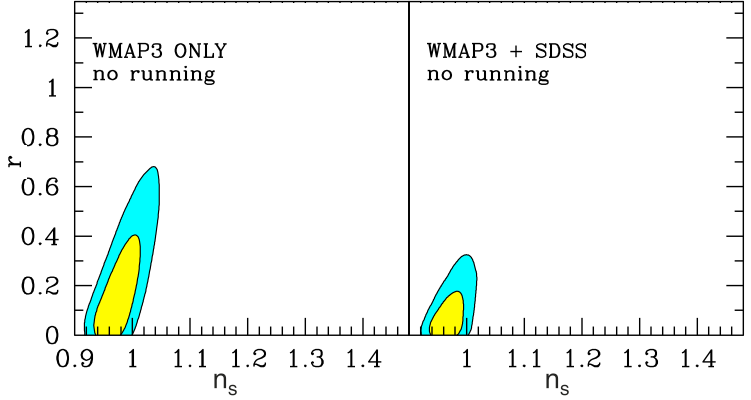
\includegraphics[trim = 1mm 1mm -1mm 0mm, clip, width=7cm, height=4.5cm]{rn.png}
  \includegraphics[trim = 1mm 1mm 3mm 10mm, clip, width=4cm, height=4.5cm]{zoonorun.pdf} 
\caption{ %Left: WMAP3 and WMAP3+SDSS data sets constrains on $n_{\rm s}$ and $r$ parameters.
WMAP3 only (open contours) and 
WMAP3+SDSS (filled contours) 2D posterior distributions on the phase space $n_{\rm s}$-$r$,
for the potentials $\phi^2$ and $\phi^4$ by considering  $e$-folds of $N\sim$ 46 and 60.
Coloured regions correspond to 68\% and 95\% CL~\citep{Kinney}.
}
\label{fig:Kinney}
\end{center}
\end{figure}

On the other hand, left panel of figure \ref{fig:Komatsu} shows limits imposed by WMAP5 data alone,   
$r < 0.43$ (95\% CL) while $0.964< n_{\rm s}<1.008$.
When BAO and SN data are added, the limits improve significantly to 
$r < 0.22$ (95\% CL) and {$0.953< n_{\rm s}<0.983$ \citep{Komatsu}}.
Right panel of figure \ref{fig:Komatsu} displays a summary for different potentials constraints by WMAP5+BAO+SN.
%On the other hand, WMAP5 results are summarised in Figure \ref{fig:Komatsu2}:
The model $V(\phi)=\lambda \phi^4$, unlike WMAP3 constraints, is found to be located 
far away from the 95\% CL, and therefore it is excluded by more than 2$\sigma$. For inflation produced by a massive 
scalar field $V(\phi)=(1/2)m^2\phi^2$, the model with $N=50$ is situated outside the 
68\% CL, whereas with $N=60$ is at the boundary of the 68\% CL. 
Therefore, this model is consistent with data within the 95\% CL. 
The points represented by $N$-flation describe a model with many massive axion fields \citep{Liddle3}. 
For an exponential potential, it is observed that models with $p<60$ are mainly excluded.
Models with $60<p<70$ are roughly in the boundary of the 95\% region, and $p>70$ are 
in agreement within the 95\% CL. 
Some models with $p\sim 120$ essentially lay out in the limit of the 68\% CL.
\\

The hybrid potentials, as already noted, can have different behaviours
depending on the $(\phi/ \mu)$ value. The parameter space can be split into three 
different regions based on $(\phi / \mu)$. For $\phi / \mu \ll 1$ the dynamics is similar to small
fields and the dominant term lays in the region called ``Flat Potential Regime". 
For $\phi / \mu \gg 1$ the results are similar to large field models and this region is called
``Chaotic Inflation-like Regime". The boundary, $\phi / \mu \sim 1$ is named 
``Transition regime". The different $(\phi / \mu)$ values corresponding to their regions
are shown in the right panel of Figure \ref{fig:Komatsu}.
Finally, the combined datasets WMAP5+BAO+SN ruled out the Harrison-Zel'dovich model
by more than 95\% CL.
\\

\begin{figure}[t!]
\begin{center}
 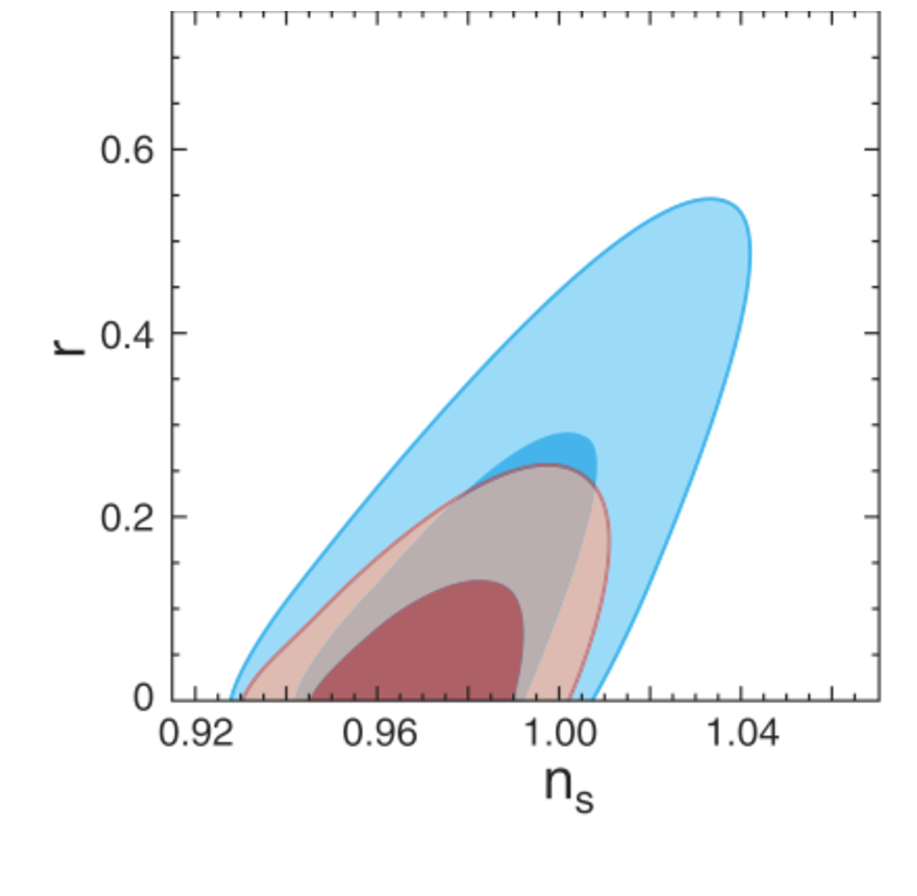
\includegraphics[trim = 1mm 10mm -2mm -10mm, clip, width=3.cm, height=4.cm]{komatsu1.pdf}
  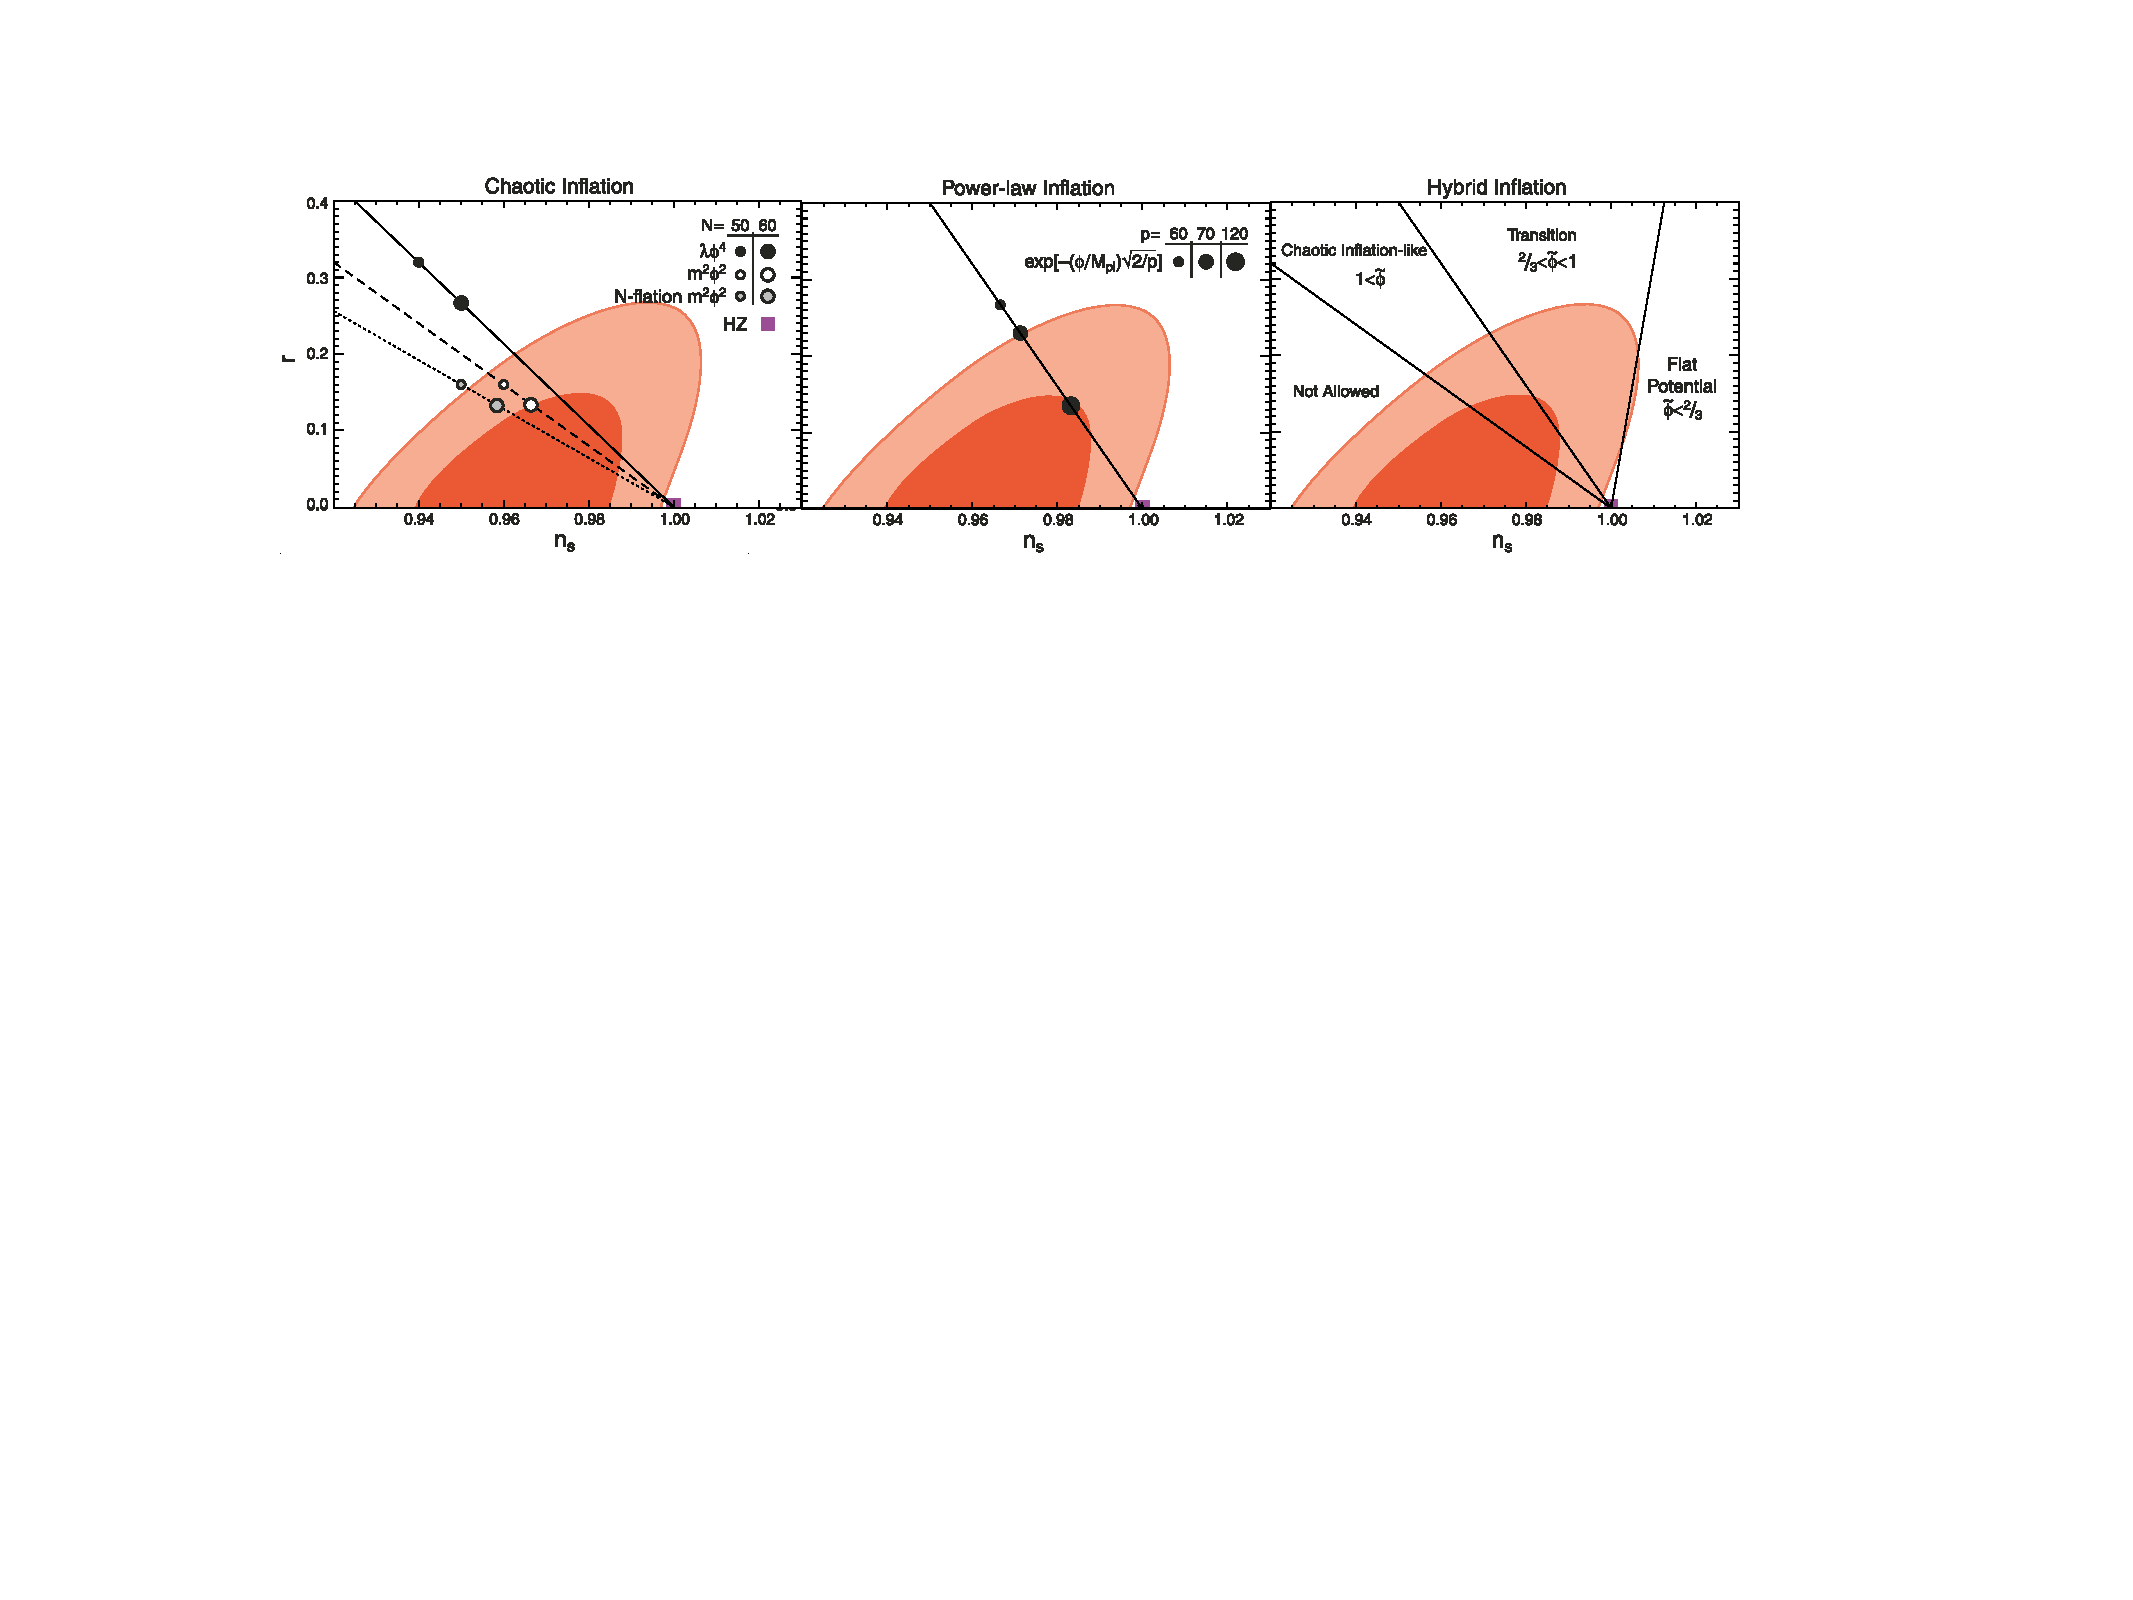
\includegraphics[trim = 0mm 0mm 2mm 0mm, clip, width=8.6cm, height=4.2cm]{komat.pdf} 
\caption{Constraints on $n_{\rm s}$ and $r$.
Left panel: WMAP5 results are coloured blue and WMAP5+BAO+SN red.
Right panel: Constraints on large and hybrid models from the combined datasets WMAP5+BAO+SN.
Coloured regions correspond to 68\% and 95\% CL
 \citep{Komatsu}.}\label{fig:Komatsu}
\end{center}
\end{figure}

Following the same line for inflationary models, we use the {\sc cosmoMC} package \citep{Lewis}
which allows us to perform the parameter estimation and to provide constraints for the $n_{\rm s}$ and $r$ parameters given 
a dataset [we refer to \citet{Padilla} where the authors provided an introduction on Bayesian parameter inference and 
its applications to cosmology].
We assume a flat $\Lambda$CDM model 
specified bythe following parameters: the physical baryon $\Omega_{\rm b} h^2$ and cold dark matter density
 $\Omega_{\rm DM } h^2$ relative to the critical density, $\theta$ is $100 \times$ the ratio of the sound horizon 
 to angular diameter distance at last scattering surface and $\tau$ denotes the optical depth at reionisation.
 %
To illustrate our point, we initially consider WMAP seven year data. 
We observe from Figure \ref{fig:infla} that in order a 
model to be considered as a favourable candidate 
it has to predict a spectral index about  $n_{\rm s}=0.982^{+0.020}_{-0.019}$ 
 and a tensor-to-scalar ratio $r<0.37$ (95\% CL).
When WMAP-7 is combined with different datasets, the constraints are tighten as it is 
shown by \citet{Larson}. 



\begin{figure}[h!]
\begin{center}
 \includegraphics[trim = 10mm 50mm 20mm 40mm, clip, width=7cm, height=5cm]{infla_wmap7.pdf}
\caption{1D and 2D Marginalised probability constraints on $n_{\rm s}$ and $r$ using only WMAP7 data. 
2D constraints are plotted with $1\sigma$ and
$2\sigma$ confidence contours
}\label{fig:infla}
\end{center}
\end{figure}	


 %Future observations will reach higher accuracy and therefore strengthen the constraints. 
 %We build a simple toy model from an optimistic Planck-like sensitivity \citep{Planck} using 
 %the best-fit parameters extracted from WMAP7 year as a fiducial values (see Figure \ref{fig:infla_2}). 
%The constraints on $n_{\rm s}$ are highly improved using this idealised experiment: $n_{\rm s}%=0.968\pm0.006$
%and $r<0.15$ with 95\% CL.

%\begin{figure}[h!]
% \begin{center}
% \includegraphics[trim = 1mm 50mm 10mm 40mm, clip, width=6cm, height=4.5cm]{planck.pdf}
%\caption{2D marginalised probability onstraints on $n_{\rm s}$ and $r$ for
%a particular realisation at Planck-like sensitivity. 2D constraints are plotted with $1\sigma$ adn $2\sigma$
%confidence contours.
%}\label{fig:infla_2}
%\end{center}
%\end{figure}	


%%%%%%%%%%%%%%%%%%%%%%%%%%%%%%%%%%%%%%%%%%
%\section{CONSTRAINTS ON INFLATIONARY MODELS}
%%%%%%%%%%%%%%%%%%%%%%%%%%%%%%%%%%%%%%%%%%%%%%%%



%\begin{figure}[h!] 
%\begin{center}
% \includegraphics[trim = 1mm 1mm 1mm 1mm, clip, width=6cm, height=4.5cm]{zoonorun.pdf} 
%\caption{WMAP3 (open contours) and 
%WMAP3+SDSS (filled contours) constraints on phase space $n_{\rm s}$, $r$. Contours with 68\% CL 
%and 95\% are shown with dashed lines \citep{Kinney}.}
%\label{fig:Kinney2}
%\end{center}
%\end{figure}


  


%\begin{figure}[h!]
%\begin{center}
% \includegraphics[trim = 0mm 0mm 0mm 0mm, clip, width=5cm, height=9cm]{komatsu2.pdf} 
%\caption{Constraints on large and hybrid models obtained from WMAP5+BAO+SN.
%They are shown in contours with 68\% and 95\% CL
% \citep{Komatsu}.}
% \label{fig:Komatsu2}
%\end{center}
%\end{figure}

Two recent experiments have placed new constraints on the cosmological parameters: the Atacama
Cosmology Telescope (ACT) \citet{ACT} and the South Pole Telescope (SPT) \citet{SPT}.
Figure \ref{fig:SPT} shows the predicted values for a chaotic inflationary model with inflaton
potential $V(\phi)\propto\phi^p$ with 60 e-folds. We observe that models with $p\ge3$
are disfavored at more than 95\% CL.
\\

\begin{figure}[h!]
 \includegraphics[trim = 1mm 1mm 1mm 1mm, clip, width=6cm, height=5cm]{ACT}
  \includegraphics[trim = 1mm 1mm 1mm 1mm, clip, width=6cm, height=5cm]{SPT}
%\centerline{ \epsfxsize=200pt \epsfbox{ACT} }
%\centerline{ \epsfxsize=200pt \epsfbox{SPT} }
\caption{Marginalized 2D probability distribution (68\% and 95\% CL) for the 
tensor-to-scalar ratio $r$, and the scalar spectral index $n_{\rm s}$ for ACT+WMAP (left panel)
and SPT+WMAP (right panel)
 \citep{ACT,SPT}.}
 \label{fig:SPT}
\end{figure}


Figure \ref{fig:infla_2}  shows recent constrains given by \citet{PlanckC} in the $n_s$ and $r$ plane. 
Gray regions correspond to the Planck 2013 results, red regions added the contribution of the temperature 
power spectrum (TT) and the Planck polarization data in the low-$l$ likelihood (lowP) while blue regions added 
the temperature-polarization cross spectrum (TE) and the polarisation power spectrum (EE).
Notice that the model that fit the best to the data corresponds to $R^2$ inflation \citep{Starobinsky}
and models $V(\phi)~\phi^p$ with $p\geq 2$ are discarded by data.
Finally, the addition of BAO data and lensing is shown in Figure \ref{fig:infla_3}.

\begin{figure}[h!]
 \begin{center}
  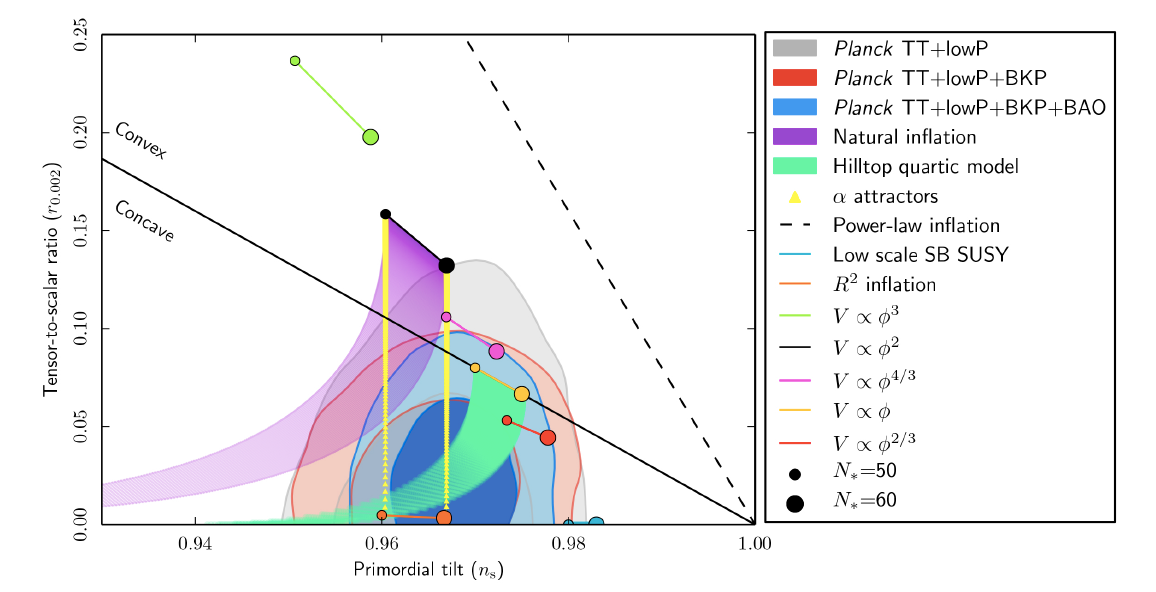
\includegraphics[trim = 1mm 1mm 1mm 1mm, clip, width=9cm, height=5cm]{Planck}
\caption{2D marginalised probability constraints on $n_{\rm s}$ and $r$ for
the most resent results of \citep{PlanckC}. 2D constraints are plotted with $1\sigma$ adn $2\sigma$
confidence contours. Figure taken from \citet{PlanckC}.
}\label{fig:infla_2}
\end{center}
\end{figure}	



%%%%%%%%%%%%%%%%%%%%%%%%%%%%%%%%%%%
\section{Conclusions}
%%%%%%%%%%%%%%%%%%%%%%%%%%%%%%%%%%%

\begin{figure}[h!]
 \begin{center}
  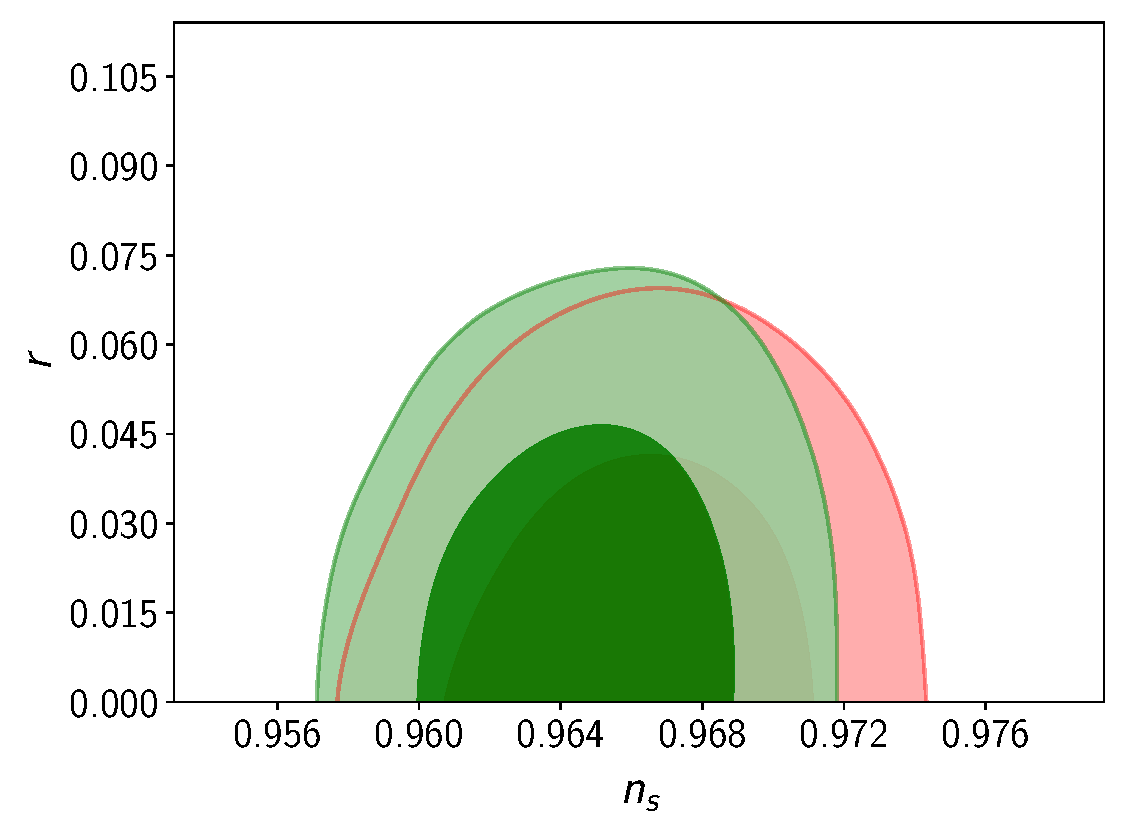
\includegraphics[trim = 1mm 1mm 1mm 1mm, clip, width=7cm, height=5cm]{inflation_rns}
\caption{2D marginalised probability constraints on $n_{\rm s}$ and $r$ for
the most resent results of Planck dataset. 2D constraints are plotted with $1\sigma$ and $2\sigma$
confidence contours. Figure done by using the CosmoMC package.
}\label{fig:infla_3}
\end{center}
\end{figure}	



\begin{table}[h!]\centering
  \setlength{\tabnotewidth}{1.0\columnwidth}
  \tablecols{3}
   \setlength{\tabcolsep}{2.8\tabcolsep}
\caption{Summarise of the \lowercase{$n_{\rm s}$, $r$} constraints from different measurements \tabnotemark{a}.}
\label{tab:resul}
\begin{tabular}{|c|c|c|}
\toprule
Parameter & Limits & Data set\\
\hline
%& & \\
$n_{\rm s}$& $ 0.9683 \pm {0.0059}$ & Planck TT + lowP + lowTE + BKP \\ 
$r$ & $< 0.0660$ & + BAO + lensing\\
\hline
$n_{\rm s}$& $ 0.9666 \pm {0.0062}$ & Planck TT+lowP\\ 
$r$ & $< 0.103$ & \\
\hline
%& & \\
$n_{\rm s}$& $ 0.9711 \pm {0.0099}$ & SPT+WMAP7+BAO+$H_0$\\ 
$r$ & $< 0.17$ & \\
\hline
%& & \\
$n_{\rm s}$& $ 0.970 \pm {0.012}$ & ACT+WMAP7+BAO+$H_0$\\ 
$r$ & $< 0.19$ & \\
\hline
%& & \\
$n_{\rm s}$& $ 0.973 \pm 0.014$ & WMAP7 + BAO +$H_0$\\ 
$r$ & $< 0.24$ & \\
\hline
%& & \\
$n_{\rm s}$& $ 0.982 \pm ^{+0.020}_{-0.019}$ & WMAP7 ONLY\\ 
$r$ & $< 0.36$ & \\
\hline
%& & \\
$n_{\rm s}$& $ 0.968 \pm 0.015$ & WMAP5+BAO+SN\\ 
$r$ & $< 0.22$ & \\
\hline
%& & \\
$n_{\rm s}$ & $0.986\pm  0.022$ & WMAP5 ONLY  \\
$r$ & $  < 0.43 $ &  \\
\hline
%& & \\
$n_{\rm s}$& $0.97\pm 0.04 $ & WMAP3 + SDSS\\ 
$ r$& $<0.31$ & \\
 \hline
%& & \\
$n_{\rm s}$& $0.99 \pm 0.05 $ & WMAP3 ONLY \\
 $r$& $< 0.60 $ &  \\
\bottomrule
\tabnotetext{a}{Peiris et al.2003; Kinney et al.2006; 
Komatsu et al.2009; Komatsu et al.2011; Dunkley et al. 2010; Keisler et al. 2011, Planckck}
\end{tabular}
%\end{ruledtabular}
\end{table}


Considering the analysis presented here is complicated to prove 
that a given model is correct, since these could be just particular cases of more general 
models with several parameters involved. However, it is possible to eliminate models 
or at least give some constraints on their behaviour leading to a narrower range of study.
%
Although we have presented some simple examples of potentials, 
the classification in small-field, large-field, and hybrid models is enough to 
cover the entire region of the $n_{\rm s}$--$r$ plane as illustrated in Figure \ref{fig:parameters}.  
Different versions of the three types of models predict qualitatively different
scalar and tensor spectra, so it should be particularly easy to work on
them apart.
\\

We have seen that the favoured models are those with small $r$ (for $dn_{\rm s}/d\ln{k}\sim 0$)
and slightly \textit{red} spectrum, hence models with \textit{blue} power spectrum  $n_s > 1.0$
are inconsistent with the recent data. These simple but important constraints allow us to rule out
the simplest models corresponding to hybrid inflation of the form 
$V(\phi) = \Lambda^4(1 + (\mu / \phi)^{p})$. There still remain models with red spectra in 
the hybrid classification: inverted models and models with logarithmic potentials. 
\\

Table \ref{tab:resul} summarises the constraints on the $n_{\rm s}$ and $r$ parameters
and its improvements through the years.
Scale-invariant power spectrum $n_{\rm s} = 1$ is consistent within 95\% CL with WMAP3 data 
%alone, considering no running of the spectral index. The HZ spectrum is 
and therefore not ruled out, however with WMAP5 data the HZ spectrum lays outside 
the 95\% CL region, which indicates it is excluded considering the lowest order 
on the $n_{\rm s}, r$ parameters. When WMAP7 data is considered, 
scale-invariant spectrum is totally excluded by more than $3 \sigma$, 
 however the inclusion of extra parameters may weaken the constraints on the spectral index.
 %, in which case ertain models are still consistent with HZ  even for current observations. 
When chaotic models $V(\phi)\propto\phi^p$ are analysed with current data, 
it is found that quartic models 
($p=4$) are ruled out, whilst models with $p\ge3$ are disfavoured at $>$ 95\% CL.
Moreover, the quadratic potential $V(\phi)= 1/2 m^2 \phi^2$ is in agreement
with all data sets presented here and therefore remains as a good candidate.
Future surveys will  provide a more accurate description of the universe and therefore 
narrow the number of candidates which might better explain the inflationary period.



\section{Acknowledgments }

LEP were supported by CONACyT M\'exico.


%%%%%%%%%%%%%%%%%%%%%%%%%%%%%%%%%%%%%%%%%%%%%%%%
%\bibliography{references}
%%%%%%%%%%%%%%%%%%%%%%%%%%%%%%%%%%%%%%%%%%%%%%%%

\begin{thebibliography}


\bibitem[Planck Colaboration(2015)]{PlanckC}Ade P. A. R.   et  al.  Planck  collaboration.  Astron.  Astrophys. 594, A20 (2016). arXiv:1502.02114

\bibitem[Albrecht \& Steinhardt(1982)]{Steinhardt} Albrecht, A., and {Steinhardt,} P.~J. 1982, \prl, 48,  1220  

\bibitem[Ambrosio(2002)]{Ambrosio02}Ambrosio, M., et~al. 2002, Eur. Phyis. J. C., 25, 511  

\bibitem[Ast. parameters(2016)]{Apar} Astrophysical Constant and Parameters,
{http://pdg.lbl.gov/2016/reviews/rpp2016-rev-astrophysical-constants.pdf}, revised December 2017

\bibitem[Barrow \& Parsons(1995)]{Barrow2}Barrow, J. D., and {Parsons}, P. 1995, Phys. Rev. D, 52, 10 
  
%\bibitem[Barrow \& Tipler(1986)]{Barrow}Barrow, J.~D., Tipler, F.~J., 1986, The Anthropic Cosmological Principle,
%  Clarendon Press, Oxford, UK 

 \bibitem[Baumann \& Peiris(2009)]{Baumann}Baumann, D., and  {Peiris,} H. V. 2009, Adv. Sci. Lett., 2, 105
%astro-ph/08103022

\bibitem[McCoy(2014)]{McCoy}C. D. McCoy, What Is the Horizon Problem?, november 2014
\bibitem[Carroll(2001)]{Carrol01}Carroll, S. 2001, Living Rev. Relativity, 3
   
\bibitem[Coles \& Lucchin(1995)]{Coles}Coles, P., and Lucchin, F. 1995, Cosmology, WILEY, England, UK 

 \bibitem[Copeland et al.(1994)]{Copeland} Copeland, E. J., et~al. 1994, Phys. Rev. D, 49, 6410
%astro-ph/93080044

\bibitem[Dodelson (2003)]{Dodelson}Dodelson, S. 2003, Modern Cosmology, Academic Press, Amsterdam, Netherlands 

  \bibitem[Dunkley et al.(2010)]{ACT}Dunkley, J.,  et al. 2010, astro-ph/1009.0866. 
 
\bibitem[Georgi \& Glashow(1974)]{Georgi}Georgi, H., Glashow, S. L. 1974, Phys. Rev. Lett., 32, 438
 
\bibitem[Gold et al.(2011)]{Gold}Gold, B., et al. 2011, ApJS, 192, 15

\bibitem[Graham(2016)]{Graham}Graham G. Ross, Gabriel German, J. Alberto Vazquez. JHEP 1605 (2016) 010

\bibitem[Guo et al.(2011)]{Guo}Guo Z.-K., D.J. Schwarz and Y.-Z. Zhang. JCAP 08 (2011) 031

\bibitem[Guth(1997)]{Guth2}Guth, A.~H. 1997, The Inflationary Universe,  Ed. Vintage
        
\bibitem[Guth(1981)]{Guth}Guth, A.~H. 1981, \prd, 23,  347 
 
\bibitem[Hinshaw et al.(2009)]{wmap5}Hinshaw, G., et~al. 2009, ApJS, 180, 225
%astro-ph/08030732 
\bibitem[R. Hlozek et al.(2012)]{Hlozek}R. Hlozek., et~al. Astrophys. J. 749 (2012) 90

\bibitem[Hu \& Dodelson(2002)]{Hu}Hu, W., and {Dodelson,} S. 2002, Annu. Rev. Astron. and Astrophys., 40, 171

  \bibitem[Keisler et al.(2011)]{SPT}Keisler, R., et al. 2011, astro-ph/1105.3182  
 
\bibitem[Kinney(2004)]{Kinney2}  Kinney, W . H. 2004, CU-TP-1083, astro-ph/0301448
 
\bibitem[Kinney et al.(2006)]{Kinney} Kinney, W. H.,  et~al. 2006, Phys. Rev. D, 74, 023502
% astro-ph/0605338 

\bibitem[Kinney \& Riotto(1998)]{Kinney3} Kinney, W.~H., and {Riotto}, A.,  1998, Phys. Lett., 435B, 272
%astro-ph/9802443

\bibitem[Kolb \& Turner(1983)]{Kolb83}Kolb, E. W., Turner, M. S. 1983, Ann Rev Nucl Part Sci. 33, 645
  
\bibitem[Kolb \& Turner(1994)]{Kolbbo}Kolb, E. W., Turner, M.S. 1994, The Early Universe, Westview Press  

 \bibitem[Komatsu(2009)]{Komatsu} Komatsu, E., et~al. 2009, ApJS., 180, 330 
%astro-ph/08030547
  
\bibitem[Komatsu et al.(2011)]{Komat}Komatsu, E., et~al. 2011, Astrophys. J. Suppl., 192, 18

  \bibitem[La \& Steinhardt(1999)]{La}La, D., and {Steinhardt}, P.J.  1999, Phys. Rev. D, 59, 064029
 
\bibitem[Larson et al.(2011)]{Larson}Larson, D., et~al. 2011, ApJS., 192, 16

\bibitem[Lasenby and Doran(2005)]{Lasenby} Phys. Rev. D 71 (2005) 063502

\bibitem[Lewis \& Bridle(2002)]{Lewis}Lewis A., and Bridle, S., 2002, Phys. Rev D, 66, 103511 
   
 \bibitem[Liddle(1999)]{Liddle2} Liddle, A. 1999, AIP Conf. Proc., 476, 11
% astro-ph/9901041

 \bibitem[Liddle(1998)]{Liddle3}Liddle, A.,  {Mazundar,} A., and {Schunck,} F. E. 1998, Phys. Rev. D, 58, 061301  
%astro-ph/08030547

\bibitem[Liddle(1999)]{Liddle}Liddle, A. 1999, An introduction to Modern Cosmology, WILEY, England, UK

\bibitem[Liddle \& Lyth(2000)]{LiddleLyth} Liddle, A.~R., and  Lyth, D.~H. 2000, Cosmological inflation and large-scale structure,
  Cambridge University Press, Cambridge, UK 

\bibitem[Liddle \& Lyth(2009)]{LiddleLyth2} Liddle, A.~R., and  Lyth, D.~H. 2009, The primordial density perturbation,
  Cambridge University Press, Cambridge, UK 
  
 \bibitem[Liddle \& Lyth(1992)]{Liddle92}Liddle, A.R. and Lyth, D.H 1992, Phys. Lett. B, 291, 39

 \bibitem[A. Riotto(2017)]{Riotto17} arXiv:hep-ph/0210162

 \bibitem[Liddle et al.(1994)]{Liddle94} Liddle, A. R., et~al. 1994, Phys. Rev. D, 50, 12
%astro-ph/0302225
  
\bibitem[Linde(1982)]{Linde}Linde, A.~D. 1982, Phys. Lett. B, 108,  389 
 
 \bibitem[Linde(1983)]{Linde2}Linde, A.~D. 1983, Phys. Lett. B, 129, 177 

\bibitem[Linde(1990)]{Lindeb} Linde, A.~D. 1990, Particle Physics and Inflationary Cosmology, Harwood Academic,
Switzerland 

 \bibitem[Linde(1991)]{Linde3}Linde, A. D. 1991, Phys. Lett. B,  259, 38
 
\bibitem[Linde(2005)]{Linde05}{Linde,} A. 2005, J.Phys.Conf.Ser., 24 
 
\bibitem[Lidsey(1997)]{Lidsey}  Lidsey, J. E., et al. 1997, Annu. Rev.Mod.Phys., 69,  373  
 
\bibitem[Lyth \& Riotto(1999)]{Lyth}Lyth, D.~H., and {Riotto,} A. 1999, Physics Reports, 314, 1

\bibitem[Lyth \& Stewart(1995)]{Lyth1}Lyth, D.~H., and {Stewat,} E.~D., 1995, Physics Rev. Lett. 75, 201, hep-ph/9502417

\bibitem[Lyth \& Stewart(1996a)]{Lyth2}Lyth, D.~H., and {Stewat,} E.~D., 1996a, Physics Rev. D 53, 1784, hep-ph/9510204

\bibitem[Mermod(2013)]{monopole}Mermod P., \textit{Magnetic monopoles at the LHC in the Cosmos}, arXiv:1305.3718 

\bibitem[Mortonson et al.(2011)]{Mortonson11}Mortonson, M. J., Peiris, H.V., and Easther, R. 2011, Phys.Rev. D, 83, 043505 
  
 \bibitem[Mukhanov \& Chibisov(1997)]{Mukhanov}Mukhanov, V. F., and {Chibisov,} G. V. 1997, JETP Letters, 33, 532
  
\bibitem[Olive(1990)]{Olive} Olive, K. ~A. 1990, Physics Reports, 190, 307   

\bibitem[Padilla et al.(2018)]{Padilla} Padilla, L. E.,et~al., to be submitted.   

\bibitem[Peiris et al.(2003)]{Peiris}Peiris, H. V., et~al. 2003, ApJS., 148, 213  
%astro-ph/0302225

\bibitem[Planck(2015-XI)]{Planckxi}Planck 2015 results. XI. CMB power spectra, likelihoods, and robustness of parameters, arXiv:1507.02704 [astro-ph.CO] 

\bibitem[Planck(2015-XIII)]{Planckck}Planck 2015 results. XIII. Cosmological parameters, arXiv:1502.01589 [astro-ph.CO]

\bibitem[Planck(2015-XVI)]{Planckxvi}Planck 2015 results. XVI. Isotropy and statistics of the CMB, arXiv:1506.07135v2 [astro-ph.CO]
 
\bibitem[Planck(2016)]{Planck}The Planck Collaboration, 2016, astro-ph/0604069. 
 
\bibitem[Riess(2009)]{Riess} Riess, A.~G., et~al. 2009, ApJ., 699, 539 
% astro-ph/0210007 

\bibitem[Riess et al.(2016)]{HST}Riess, Adam G., et~al. 2016,  astro-ph/1604.01424

\bibitem[Smooth et al.(1992)]{Smooth}Smooth, G. F., et~al. 1992, ApJ Letters, 396, L1 
  
\bibitem[Springel et al.(2005)]{Sping} Springel, V., et~al.  2005, Nature, 435, 629  

\bibitem[Starobinsky(1980)]{Starobinsky} Starobinsky, A.A (1980), Physics Letters B. 91: 99?102  

\bibitem[Tegmark  et al.(2001)]{Teg}Tegmark, M., et~al. 2001, Phys. Rev. D, 63, 043007   

\bibitem[Ligo colaboration(2017)]{ligo}The LIGO Scientific Collaboration and The Virgo Collaboration, \textit{A gravitational-wave standard siren measurement of the Hubble constant}
 
 \bibitem[Vilenkin \& Shellard(2000)]{Vilenkin}Vilenkin, A., Shellard, E. P. S. 2000, Cosmic Strings and Other Topological Defects,
Cambridge University Press,  Cambridge, UK 

\bibitem[Vazquez et al.(2012a)]{Vazquez1}Vazquez J. Alberto, et~al. MNRAS 442:1948-1956, 2012

\bibitem[Vazquez et al.(2012b)]{Vazquez2} Vazquez J. Alberto, et~al.  JCAP 06 (2012) 006

\bibitem[Vazquez et al.(2013)]{Vazquez3} Vazquez J. Alberto, et~al. JCAP, 08, 001 2013


%astro-ph/1001.4538

\end{thebibliography}


\end{document}
